% $Author$ $Date$
% http://www.cns.gatech.edu/~predrag/papers/atlas12.pdf

% siminos/atlas/atlas12.tex    pdflatex atlas12
%     then:    pdflatex atlas12; bibtex atlas12; pdflatex atlas12; pdflatex atlas12
% for public version, toggle \draftfalse in setupAtlas.tex
%     (that removes all comments, the blog)

\documentclass[aip,cha,reprint,
secnumarabic,
nofootinbib, tightenlines,
nobibnotes, showkeys, showpacs,
groupedaddress
%preprint,%
%author-year,%
%author-numerical,%
]{revtex4-1}
% aip,cha,preprint,numerical, nofootinbib,
% You should use BibTeX and apsrev.bst for references
% Choosing a journal automatically selects the correct APS
% BibTeX style file (bst file), so only uncomment the line
% below if necessary.
%\bibliographystyle{apsrev4-1}

\newcommand{\version}{atlas ver. 0.9, Apr 17 2012}
% Predrag on inv. subspaces ver. 0.9, Apr 17 2012}
% Predrag 					ver. 0.8, Apr 16 2012}
% Predrag Chaos J submit.   ver. 0.7, Apr 16 2012}
% Predrag 					ver. 0.6, Apr 14 2012}
% Predrag 					ver. 0.5, Apr 11 2012}
% Predrag 					ver. 0.4, Mar 10 2012}
% Predrag 					ver. 0.3, Mar 10 2012}
% Predrag 					ver. 0.2, Dec 10 2011}
% Predrag 					ver. 0.1, Apr 28 2011}

        \input setupAtlas
        \input ../inputs/def
        \input defAtlas

\begin{document}

\title[High-dimensional cartography]
{Cartography of high-dimensional flows: A visual guide to sections and slices}

%Predrag 2012-04-12: Continuous symmetry reduction of high-dimensional flows
%                    by the method of slices
%Predrag 2012-04-11: How to cut and slice a symmetry
%Predrag 2012-04-11: Have a symmetry? How to cut and slice it
%PC, until 2012-03-19: "Continuous symmetries, and how to slice them"

\author{Predrag Cvitanovi{\'c}}
\email{predrag@gatech.edu.}
\author{Daniel Borrero-Echeverry}
\author{Keith M. Carroll}
\author{Bryce Robbins}
\author{Evangelos Siminos}
\author{Lei Zhang}
\affiliation{
 Center for Nonlinear Science and School of Physics,
 Georgia Inst. of Technology,
 Atlanta, GA  30332, USA
}

\date{\today}
%\date{18 December 2011}
%\setcounter{page}{1}

    \begin{abstract}
Symmetry reduction by the method of slices quotients the continuous
symmetries of chaotic flows by replacing the original state space by a
set of charts, each covering a neighborhood of
        \PCedit{
a dynamically important class of solutions, qualitatively captured by a
`template'. Together these charts provide an atlas of the slice, charting
the regions of the manifold explored by the trajectories of interest.
    }
Within the slice, relative
equilibria reduce to equilibria, and relative periodic orbits reduce to
periodic orbits. Visualizations of these solutions and their unstable
manifolds reveal their interrelations and the role they play in
organizing turbulence / chaos.
    \end{abstract}

\pacs{02.20.-a, 05.45.-a, 05.45.Jn, 47.27.ed, 47.52.+j, 83.60.Wc}
%% showpacs class option if PACS display desired
%% copied from siminos/blog/strategy.tex
% \PACS 02.20.-a \sep 05.45.-a \sep 05.45.Jn \sep 47.27.ed \sep 47.52.+j
% 02.20.-a      Group theory, mathematics
% 05.45.-a      Nonlinear dynamics and chaos
% 05.45.Jn      High-dimensional chaos
% 47.27.ed      Dynamical systems approaches (turbulent flows)
% 47.52.+j      Chaos in fluid dynamics
% 83.60.Wc      Flow instabilities
% 95.10.Fh      Chaotic dynamics

\keywords{
symmetry reduction,
equivariant dynamics,
relative equilibria,
relative periodic orbits,
slices,
moving frames
}%Use showkeys class option if keyword display desired
\maketitle

    \begin{quotation}
Today, it is possible to take a stroll through 61,506 dimensional
\statesp\ of hydrodynamic turbulence. Charting this world is a geometer's
task, and we will map it using a measuring tape, but first one has to
deal with symmetries. Physicists have come to love them inordinately, but
Nature less so: even though the governing equations are symmetric,
turbulence breaks all symmetries, and for nonlinear systems, rather than
simplifying our task, symmetries obscure the essential dynamics. While
evolution in time decomposes the \statesp\ into a spaghetti of time
trajectories, continuous spatial symmetries stratify it like the layers
of an onion. In this geometrical tour of dynamics, we unravel this tangle
and pick a single representative point for each trajectory (section it)
and  group orbit (slice it). Once the fog of symmetries is out of the
way, one can identify and describe the prominent fluid structures by a
taxonomy of its invariant building blocks: numerically exact solutions of
\NSe, finite sets of \reqva\ and infinite hierarchies of \rpo s, and
describe the dynamics in terms of their heteroclinic connections.
    \end{quotation}

\section{Introduction}
\label{s:intro}

Over the last decade, new insights into the dynamics of moderate
\Reynolds\ turbulent flows have been gained through visualizations of
their $\infty$-dimensional \statesp s by means of dynamically invariant,
representation independent coordinate frames\rf{GHCW07} constructed from
physically prominent unstable {\cohStr s}, hereafter referred to as {\em
\template s}.
The most recent advance within this new framework is the first
determination of \rpo s that help shape the turbulence observed in pipe
flows.\rf{ACHKW11} Navigating and charting the geometry of these
extremely high-dimensional \statesp s necessitates a reexamination of two
of the basic tools of the theory of dynamical systems: \PoincSec s and
symmetry reduction.\rf{rowley_reconstruction_2000,BeTh04,SiCvi10,FrCv11}

In quantum-mechanical calculations one always starts out by making sure
that the Hamiltonian has been brought to its block-diagonal, irreducible
representation, anything else would be sheer masochism. The dynamical
theory of turbulence is still in its infancy, and symmetry reduction is
not yet common practice in numerical simulations and experimental data
collection for such strongly nonlinear systems. We show here how to bring
the numerical / experimental data to a symmetry-reduced format,
\emph{before} any analysis of it takes place. We strive to explain the
key geometrical ideas in simple but illustrative settings, eschewing the
fluid dynamical and group theoretical technicalities.

%%%%%%%%%%%%%%%%%%%%%%%%%%%%%%%%%%%%%%%%%%%%%%%%%%%%%%%%%%%%%%%%%%%%%
\begin{figure}
   \centering
  \setlength{\unitlength}{0.20\textwidth}
(a)~~~
  \begin{picture}(1,0.98239821)%
    \put(0,0){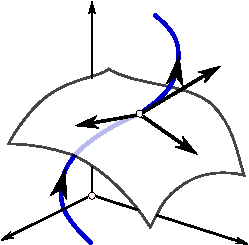
\includegraphics[width=\unitlength]{A28tangent3}}%
    \put(0.91612064,0.70682767){\color[rgb]{0,0,0}\makebox(0,0)[lb]{\smash{$\vel$}}}%
    \put(0.48698745,0.90266503){\color[rgb]{0,0,0}\makebox(0,0)[lb]{\smash{$\ssp(\zeit)$}}}%
    \put(0.2624318,0.5347756){\color[rgb]{0,0,0}\makebox(0,0)[lb]{\smash{$\groupTan_1$}}}%
    \put(0.80471037,0.38188675){\color[rgb]{0,0,0}\makebox(0,0)[lb]{\smash{$\groupTan_2$}}}%
    \put(0.538343,0.25344355){\color[rgb]{0,0,0}\makebox(0,0)[lb]{\smash{$\LieEl\ssp$}}}%
    \put(0.47864531,0.56060893){\color[rgb]{0,0,0}\makebox(0,0)[lb]{\smash{$\ssp$}}}%
  \end{picture}%
~~(b)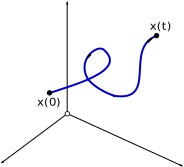
\includegraphics[width=0.20\textwidth]{A27traj}
\\
(c)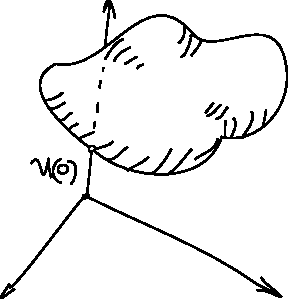
\includegraphics[width=0.20\textwidth]{A27gOrbit}
(d)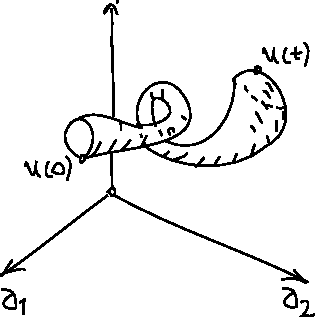
\includegraphics[width=0.20\textwidth]{A27wurst}
   \caption{\label{fig:A27wurst}
   (a)
In the presence of an $N$-continuous parameter symmetry, each \statesp\ point
$\ssp$ owns $(N\!+\!1)$ tangent vectors: one $\vel(\ssp)$ along the time
flow $\ssp(\zeit)$, and the $N$ group tangents  $\groupTan_1(\ssp), \,
\groupTan_2(\ssp) ,\,\cdots, \groupTan_N(\ssp)$ along infinitesimal
symmetry shifts, tangent to the group orbit $\LieEl\ssp$.
    (b)
Trajectory.
    (c)
Group orbit.
    (d)
Wurst.
}
\end{figure}
%%%%%%%%%%%%%%%%%%%%%%%%%%%%%%%%%%%%%%%%%%%%%%%%%%%%%%%%%%%%%%%%%%%%%

Let us begin by defining a {dynamical system} compromised of a flow $\map^t$ and the \statesp\ $\pS$ on which it acts.
If a group $\Group$ of continuous transformations
acts on a continuous time flow, each \statesp\ point owns a set of
tangent vectors (\reffig{fig:A27wurst}\,(a)). Integrated in time, the
velocity vector $\vel(\ssp)$ traces out a {\em trajectory}
$\flow{\zeit}{\ssp}$ (\reffig{fig:A27wurst}\,(b)). Applying the continuous
transformations traces out a {group orbit}
\(
\pS_\ssp = \{\LieEl\,\ssp \mid \LieEl \in {\Group}\}
% \,,\qquad \pS_\ssp \subset \pS
\,
\) %ee{sspOrbit}
(\reffig{fig:A27wurst}\,(c)). Together, time evolution and group actions trace out a complicated smooth
manifold (hereafter affectionately referred to as a {\em \wurst}, (see
Figs.~\ref{fig:A27wurst}\,(d), \ref{fig:CLf01group}\,(b) and
\ref{fig:sliceimage}) which we shall here teach you how to slice.

A flow is said to have symmetry $\Group$ if the form of evolution
equations $\dot{\ssp} = \vel(\ssp)$ is left invariant,
\(
\vel(\ssp)=\LieEl^{-1} \, \vel(\LieEl \, \ssp)
% \,,\qquad \mbox{for all }
\,,
\) %ee{eq:FiniteRot}
by the set of transformations $\LieEl \in {\Group}$. Physicists love
symmetry,\rf{Kerswell12} but Nature does not care: turbulence breaks all
symmetries, and while the flow equations may be invariant under $\Group$,
their solutions typically are not.

We can make headway in unraveling the spaghetti
of 1\dmn\ trajectories with the notion of recurrence. To quantify how
close the state of the system at a given time is to a previously
visited state, we need the notion of distance between two points in
\statesp. The simplest (but far from the only, or the most natural) is
the Euclidean norm
\beq
  \Norm{\ssp-\ssp'}^2  = \braket{\ssp-\ssp'}{\ssp-\ssp'} =
\sum_j^d
(\ssp-\ssp')_j^2
\,.
\ee{innerproduct}
    \PCedit{
For experimental data, a better norm might be a distance between digitized
images. While in this paper we simply assume that a norm is given, its
importance cannot be overemphasized: the construction of invariant, PDE
discretization independent \statesp\ charts,\rf{GHCW07} the symmetry
reduction by minimization of the distance between group orbits undertaken
in what follows, and the utility of the charts so constructed all depend on a
well-chosen notion of distance in the high-dimensional \statesp s we are
charting here.
    }

Given a notion of distance, we can talk about a `neighborhood,' an open
set of nearby states with qualitatively similar dynamics. Our main task
in what follows will be to make this precise by defining a chart over a
neighborhood and its borders. Given distances and neighborhoods, the next
key notion is  \emph{measure}, or how likely a typical trajectory is to
visit a given neighborhood. After some observations of a given turbulent
flow, one can identify a set of representative \emph{\template
s},\rf{rowley_reconstruction_2000} {points} $\slicep{}^{(j)}$,
$j=1,2,\cdots$ in the \statesp\ that are the most dynamically important
and the most frequently revisited features of the flow.

Our goals here are two-fold:
(i) In \refsect{s:cut}, we review the method of \PoincSec s, with
    emphasis on two particular aspects that are applicable to high-dimensional flows:
    the construction of multiple local linear charts and the determination of
    their borders.
(ii) In \refsect{s:symm}, we discuss the effect of continuous symmetries on
    nonlinear flows, and in \refsect{s:slice} we use the lessons learned
    from our discussion of \PoincSec s to aid us in the reduction of
    continuous symmetries, and, thus, enable us to commence a systematic
    charting of the long-time dynamics of high-dimensional flows
    (\refsect{s:chart}).


\section{Section}
\label{s:cut}

In the {\em \PoincSec} method, one records the coordinates $\sspRed_n$ of
the trajectory $\ssp(\zeit)$ at the instants $\zeit_n$ when it traverses
a fixed oriented hypersurface $\PoincS$ of codimension 1. For the
high-dimensional flows that we have in mind the practical choice is a
hyperplane, the only type of \PoincSec\ (from now on, just a
\emph{section}) that we shall consider here. One can choose a section
such that it contains a \template\ of interest. Properly oriented, such a
section can capture important features of the flow in the neighborhood of
the section-fixing \template.

But how far does this neighborhood extend? The answer is that
the section captures neighboring trajectories as long as it cuts them
transversally; it fails the moment the velocity field at a point
$\sspRSing$ fails to pierce the section. At these locations, the velocity
either vanishes (\eqv) or is orthogonal to the section normal $\hat{n}$,
\beq
    \hat{n} \cdot \vel(\sspRSing) = 0
\,,\qquad
    \sspRSing \in \cal{S}
\,.
\ee{eq:sspRSing}
For a smooth flow such points form a smooth $(d\!-\!2)$\dmn\
\emph{\poincBord} ${\cal S} \subset \PoincS$, which encloses the open
neighborhood of the {\template} characterized by qualitatively similar
flow. We shall refer to this region of the section as a chart of the
{\template} neighborhood (see \reffig{fig:RoessTrjs}\,(b) and
\reffig{fig:RoessFarEq}). Beyond the border, the flow pierces the section in the `wrong' direction and the dynamics are qualitatively
different.

As an example consider the R\"ossler system\rf{ross},
\index{R\"ossler system}
\beq
\begin{split}
  \dot{x} &= -y \,-\,z \\
  \dot{y} &= x + a y \\
  \dot{z} &= b + z (x - c)
  \,,
  \label{eq:Rossler}
\end{split}
\eeq
where $a = b = 0.2$ and $c = 5.7$. This flow has two prominent invariant
states, the `inner' and the `outer' unstable \eqva\ $\slicep{}^{(-)}$
and $\slicep{}^{(+)}$ (see \refFig{fig:RoessTrjs}\,(a)) , which we choose as {\em \template s}
 for our sections.

We orient the sections so the plane $\PoincS_{-}$ contains the 1\dmn\
stable eigenvector of $\slicep{}^{(-)}$ (\reffig{fig:RoessTrjs}\,(b)),
and the other section $\PoincS_{+}$ contains the 1\dmn\ unstable
eigenvector of $\slicep{}^{(+)}$ (\reffig{fig:RoessFarEq}\,(a)), thus
capturing the local spiral-in, spiral-out dynamics. The remaining freedom
to rotate each section can be used to orient them in such a way that the
ridge (the intersection of the two sections) lies approximately
between the two templates (\reffig{fig:RoessFarEq}\,(b)). Keep in mind that choosing sections is a dark art: in the example at hand the dynamics of interest is well captured by these two charts - if that were not the
case, one might have to interpolate, by inserting a third chart between them.

%%%%%%%%%%%%%%%%%%%%%%%%%%%%%%%%%%%%%%%%%%%%%%%%%%%%%%%%%%%%%%%%%%%%%
\begin{figure}
(a)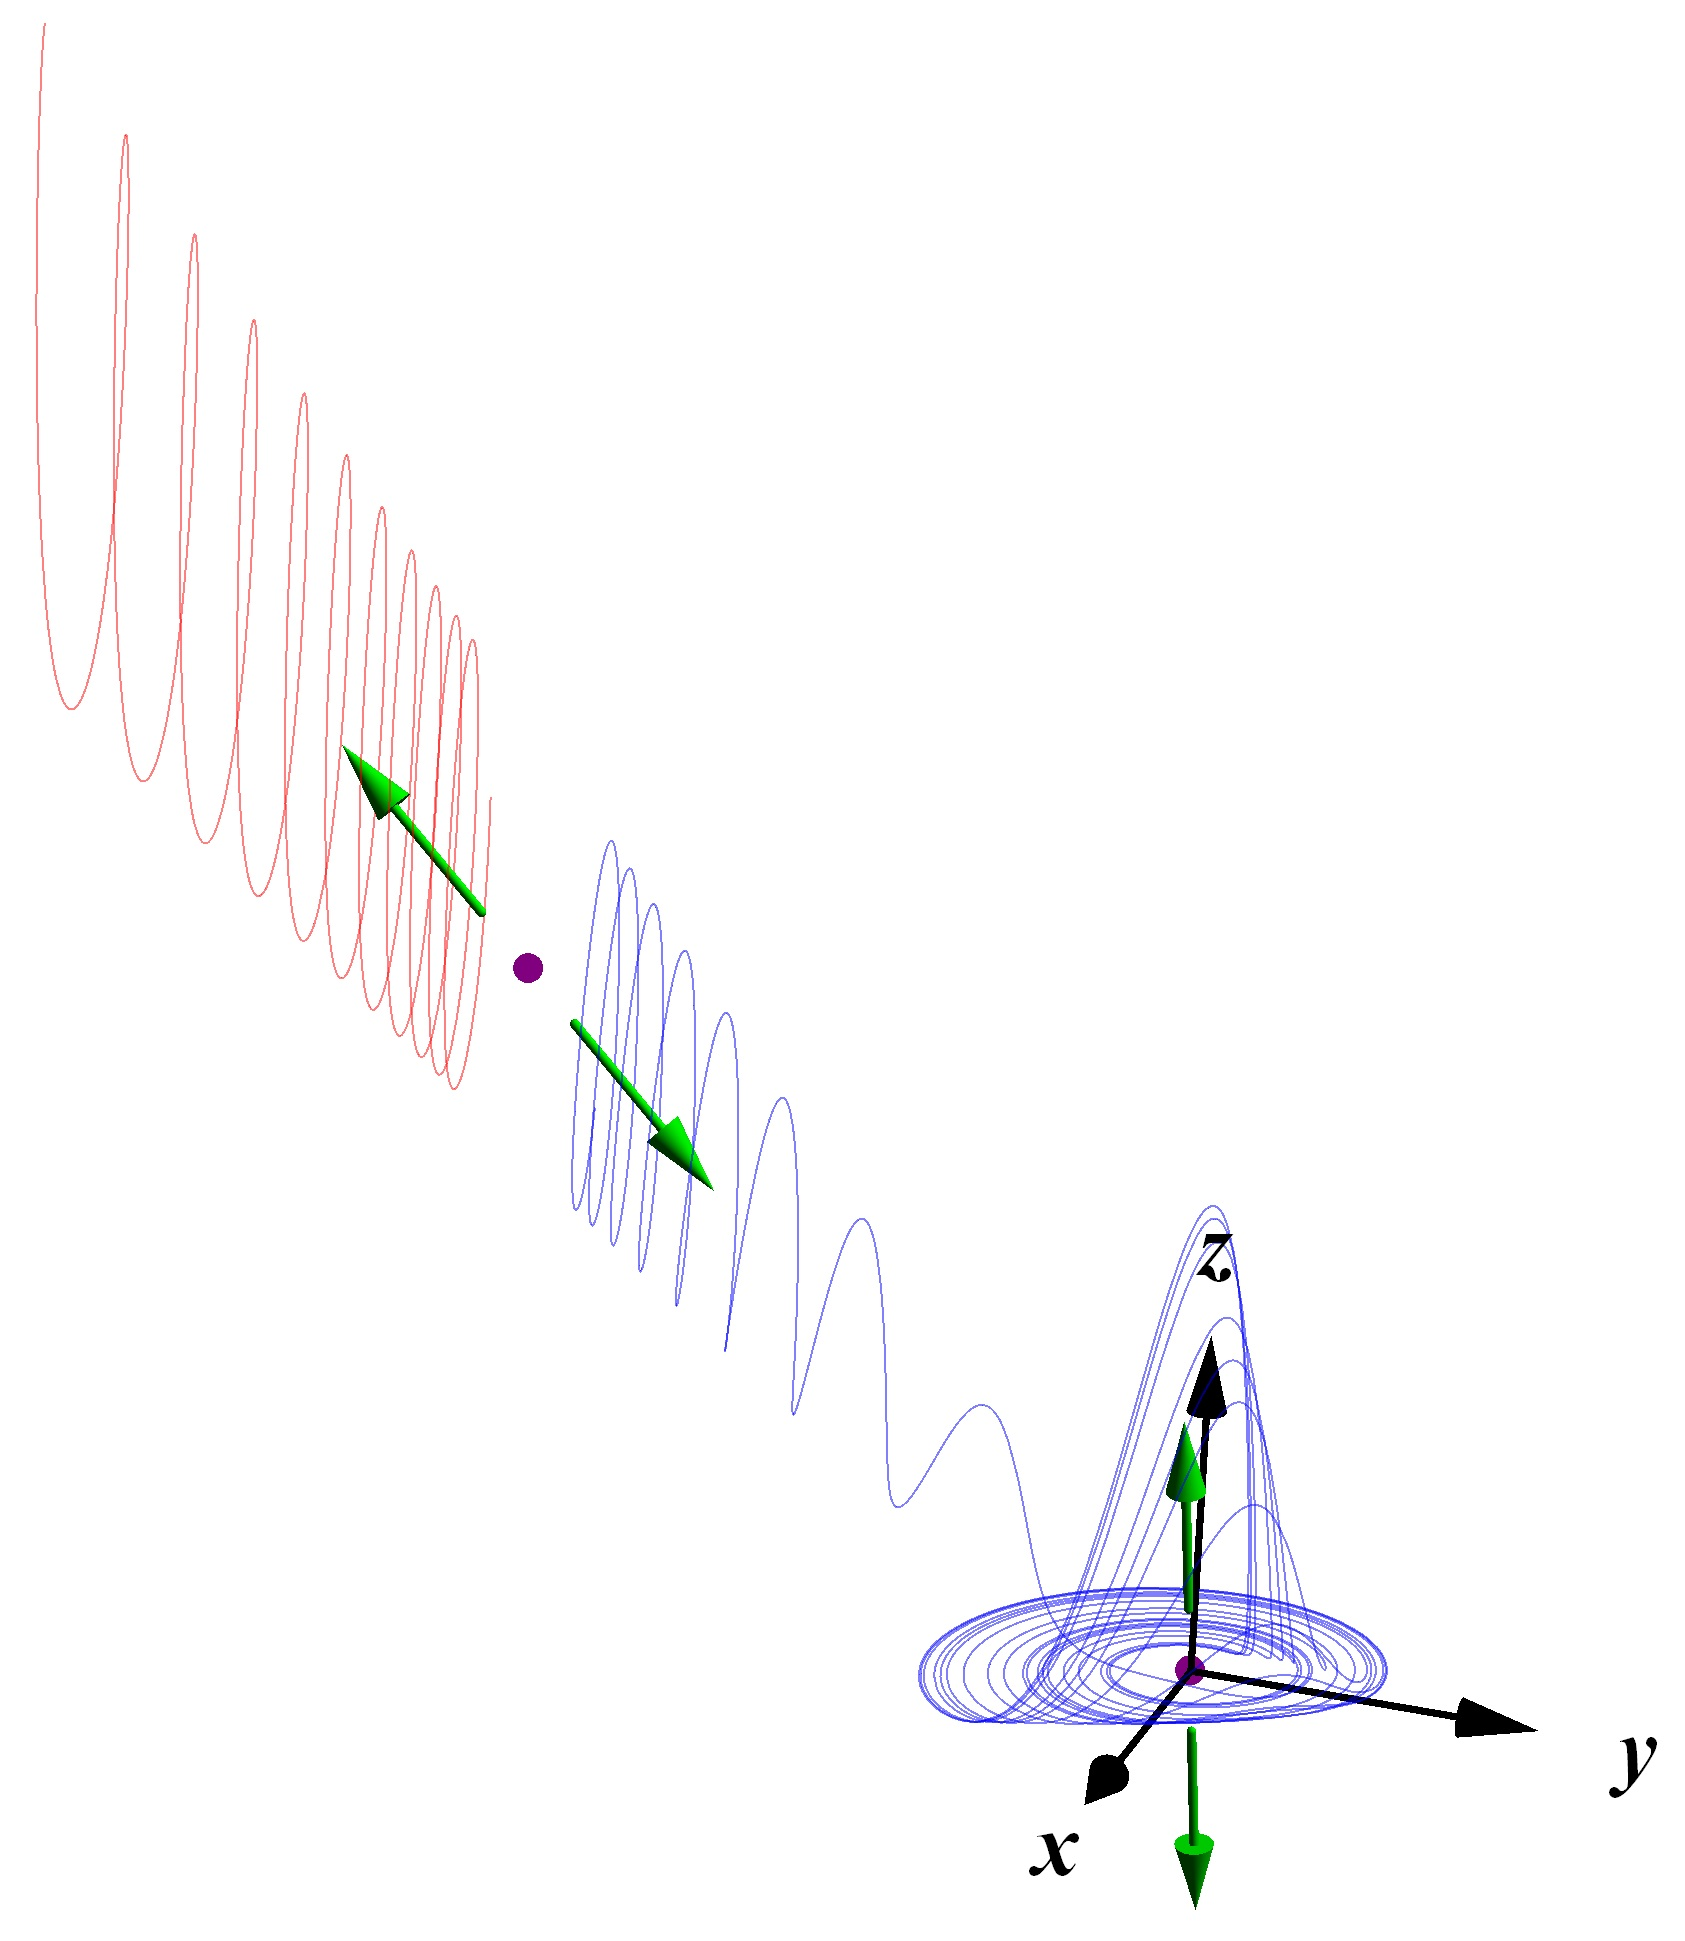
\includegraphics[width=0.28\textwidth]{RoessTrjs2}%{Rossler_Equilibria2}{RoessTrjs}%
(b)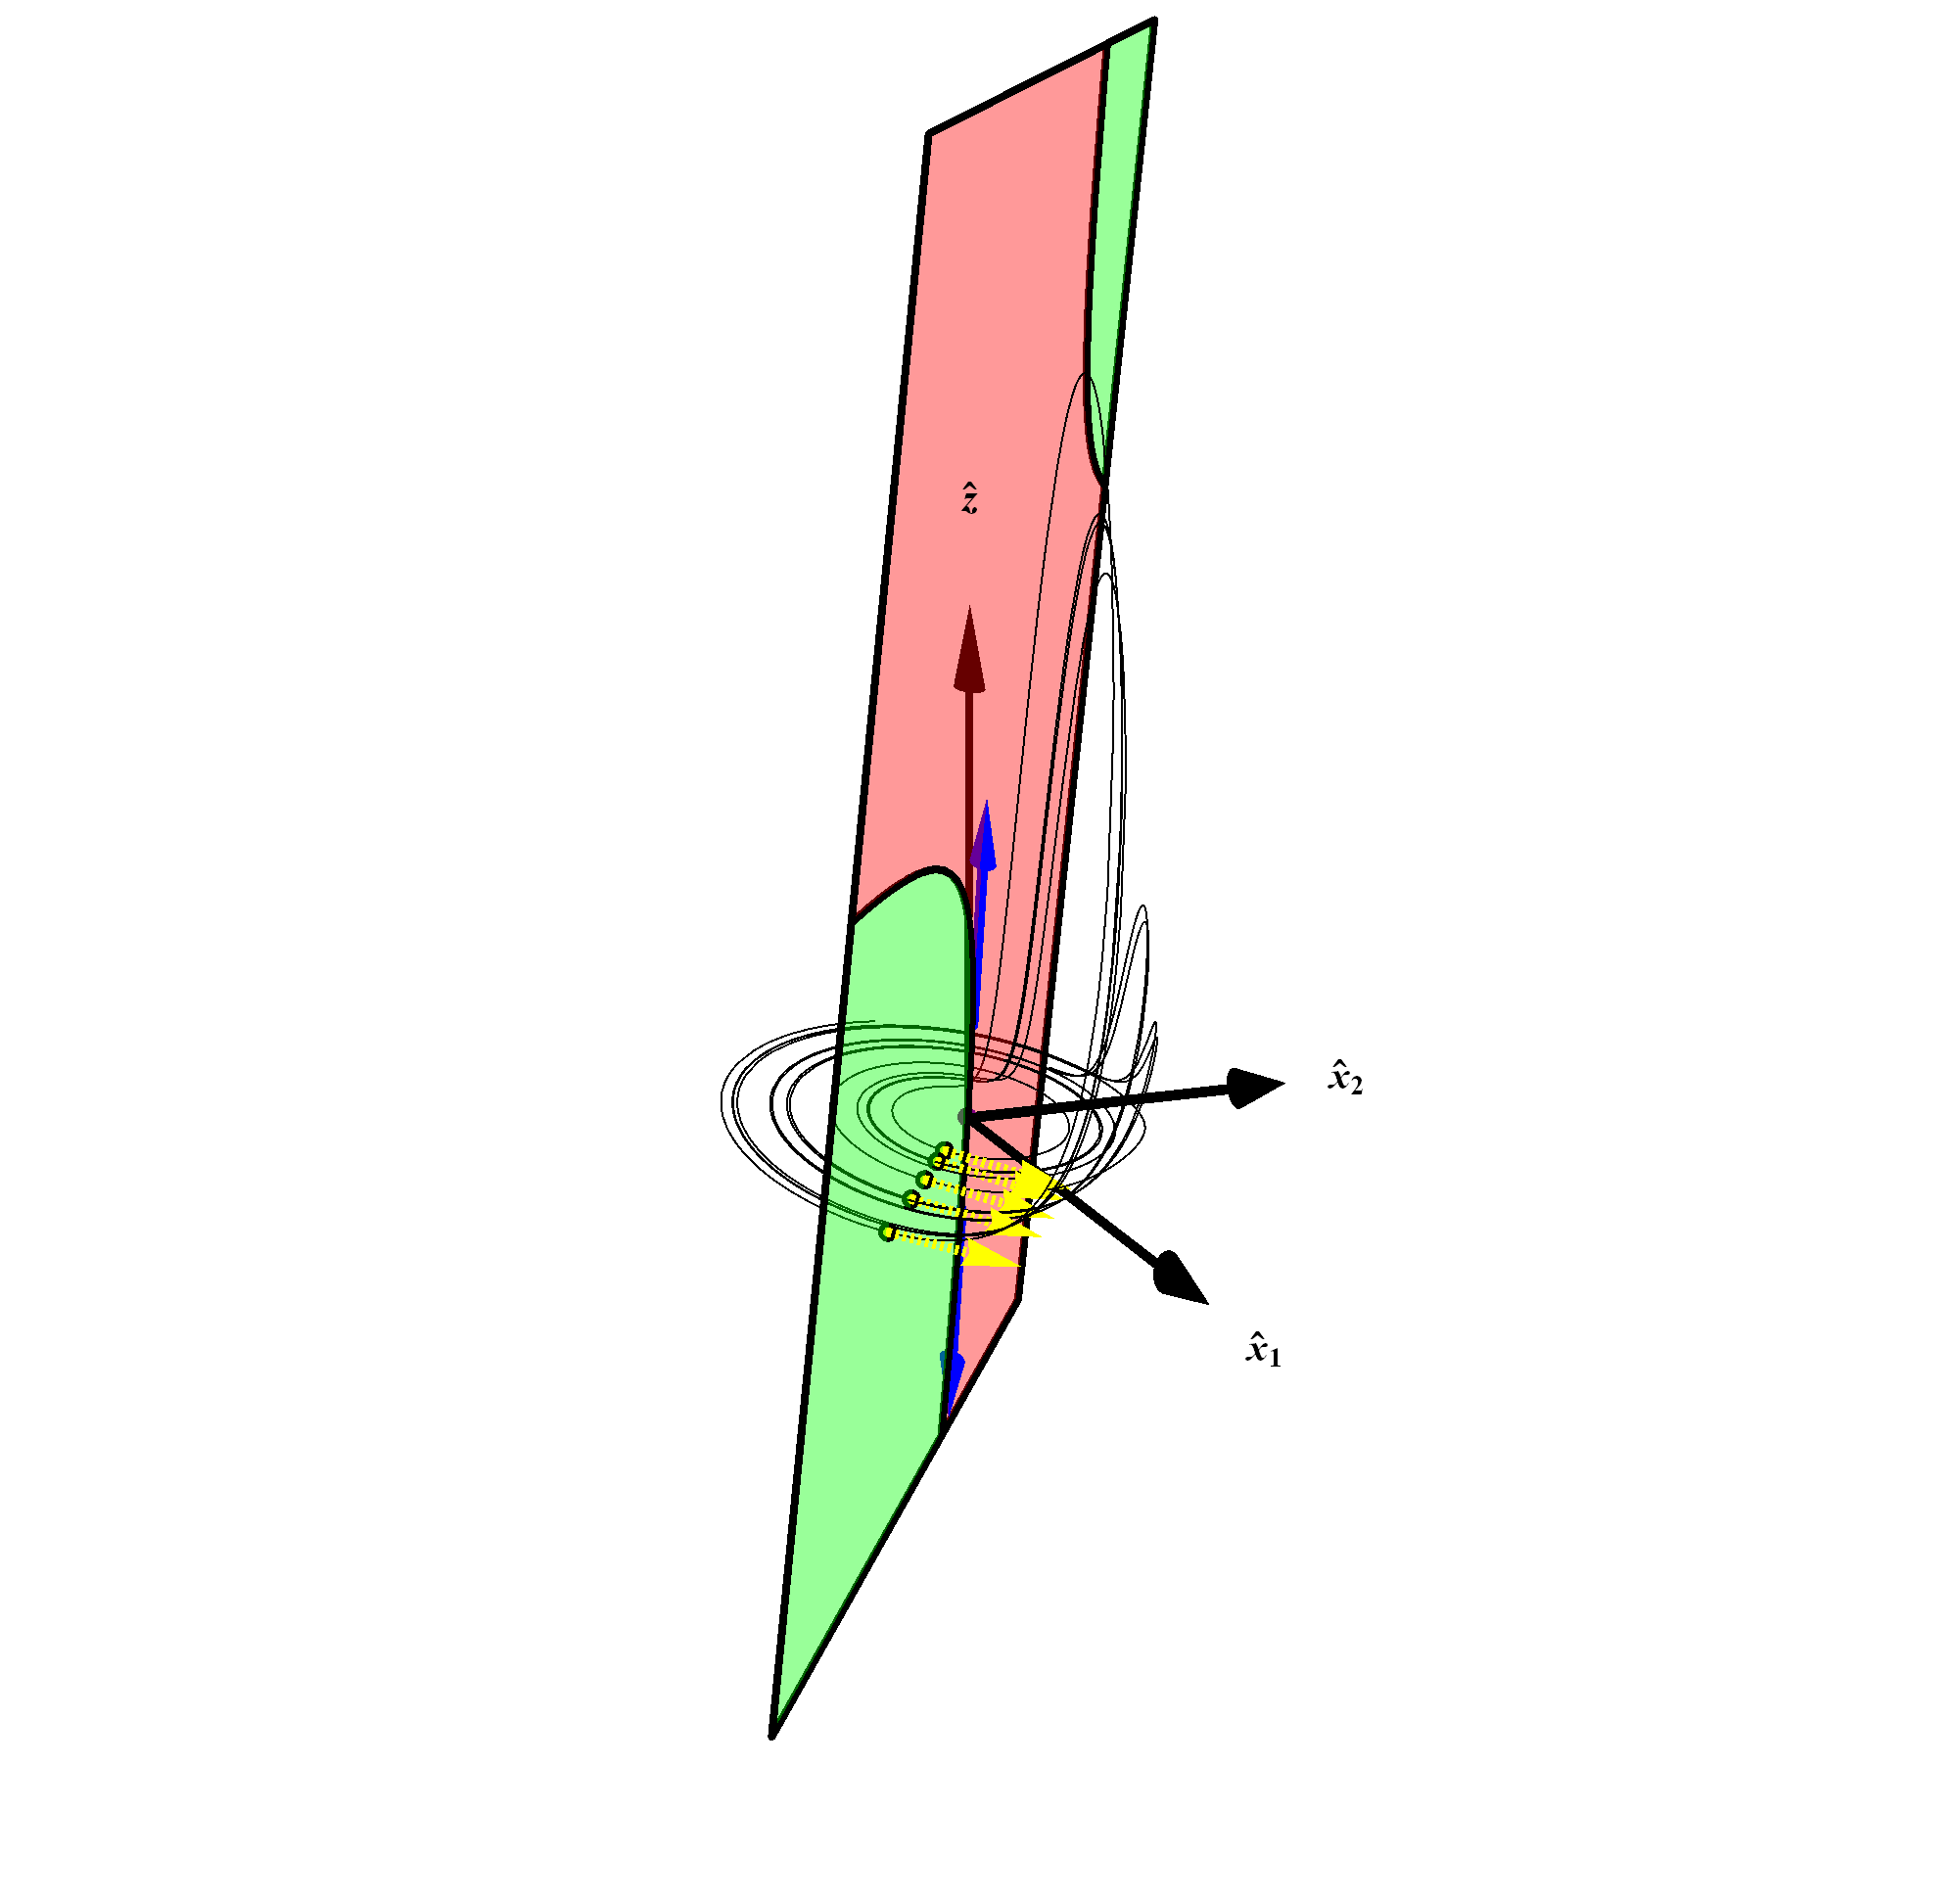
\includegraphics[width=0.14\textwidth,clip=true]{RoessNearEq3}
    \caption{
(a)
R\"ossler \eqva\ and their invariant manifolds. The stable manifold of
the inner {\eqv} $\slicep{}^{(-)}$  is 1-dimensional and its unstable one
is a spiral-out focus. For the outer {\eqv} $\slicep{}^{(+)}$,  the stable
manifold is a spiral-in focus (basin boundary for initial conditions that
either fall into the chaotic attractor, or escape to infinity) and the
unstable manifold is 1-dimensional. Shown are two trajectories near
\eqv\ $\slicep{}^{(+)}$, on spiraling outward along its unstable
manifold, and the other spiraling inward along the stable manifold of
\eqv\ $\slicep{}^{(-)}$ towards the chaotic attractor.
(b)
\PoincSec\ plane through the inner {\eqv} $\slicep{}^{(-)}$ and
its stable eigenvector. The chart $\PoincS_{-}$ of the $\slicep{}^{(-)}$
neighborhood, bounded by its \poincBord, is highlighted in light green.
    }
\label{fig:RoessTrjs}
\end{figure}
%%%%%%%%%%%%%%%%%%%%%%%%%%%%%%%%%%%%%%%%%%%%%%%%%%%%%%%%%%%%%%%%%%%%%

%%%%%%%%%%%%%%%%%%%%%%%%%%%%%%%%%%%%%%%%%%%%%%%%%%%%%%%%%%%%%%%%%%%%%
% supercedes \label{fig:RoessBothEq}
\begin{figure}%[H]
\begin{center}
(c)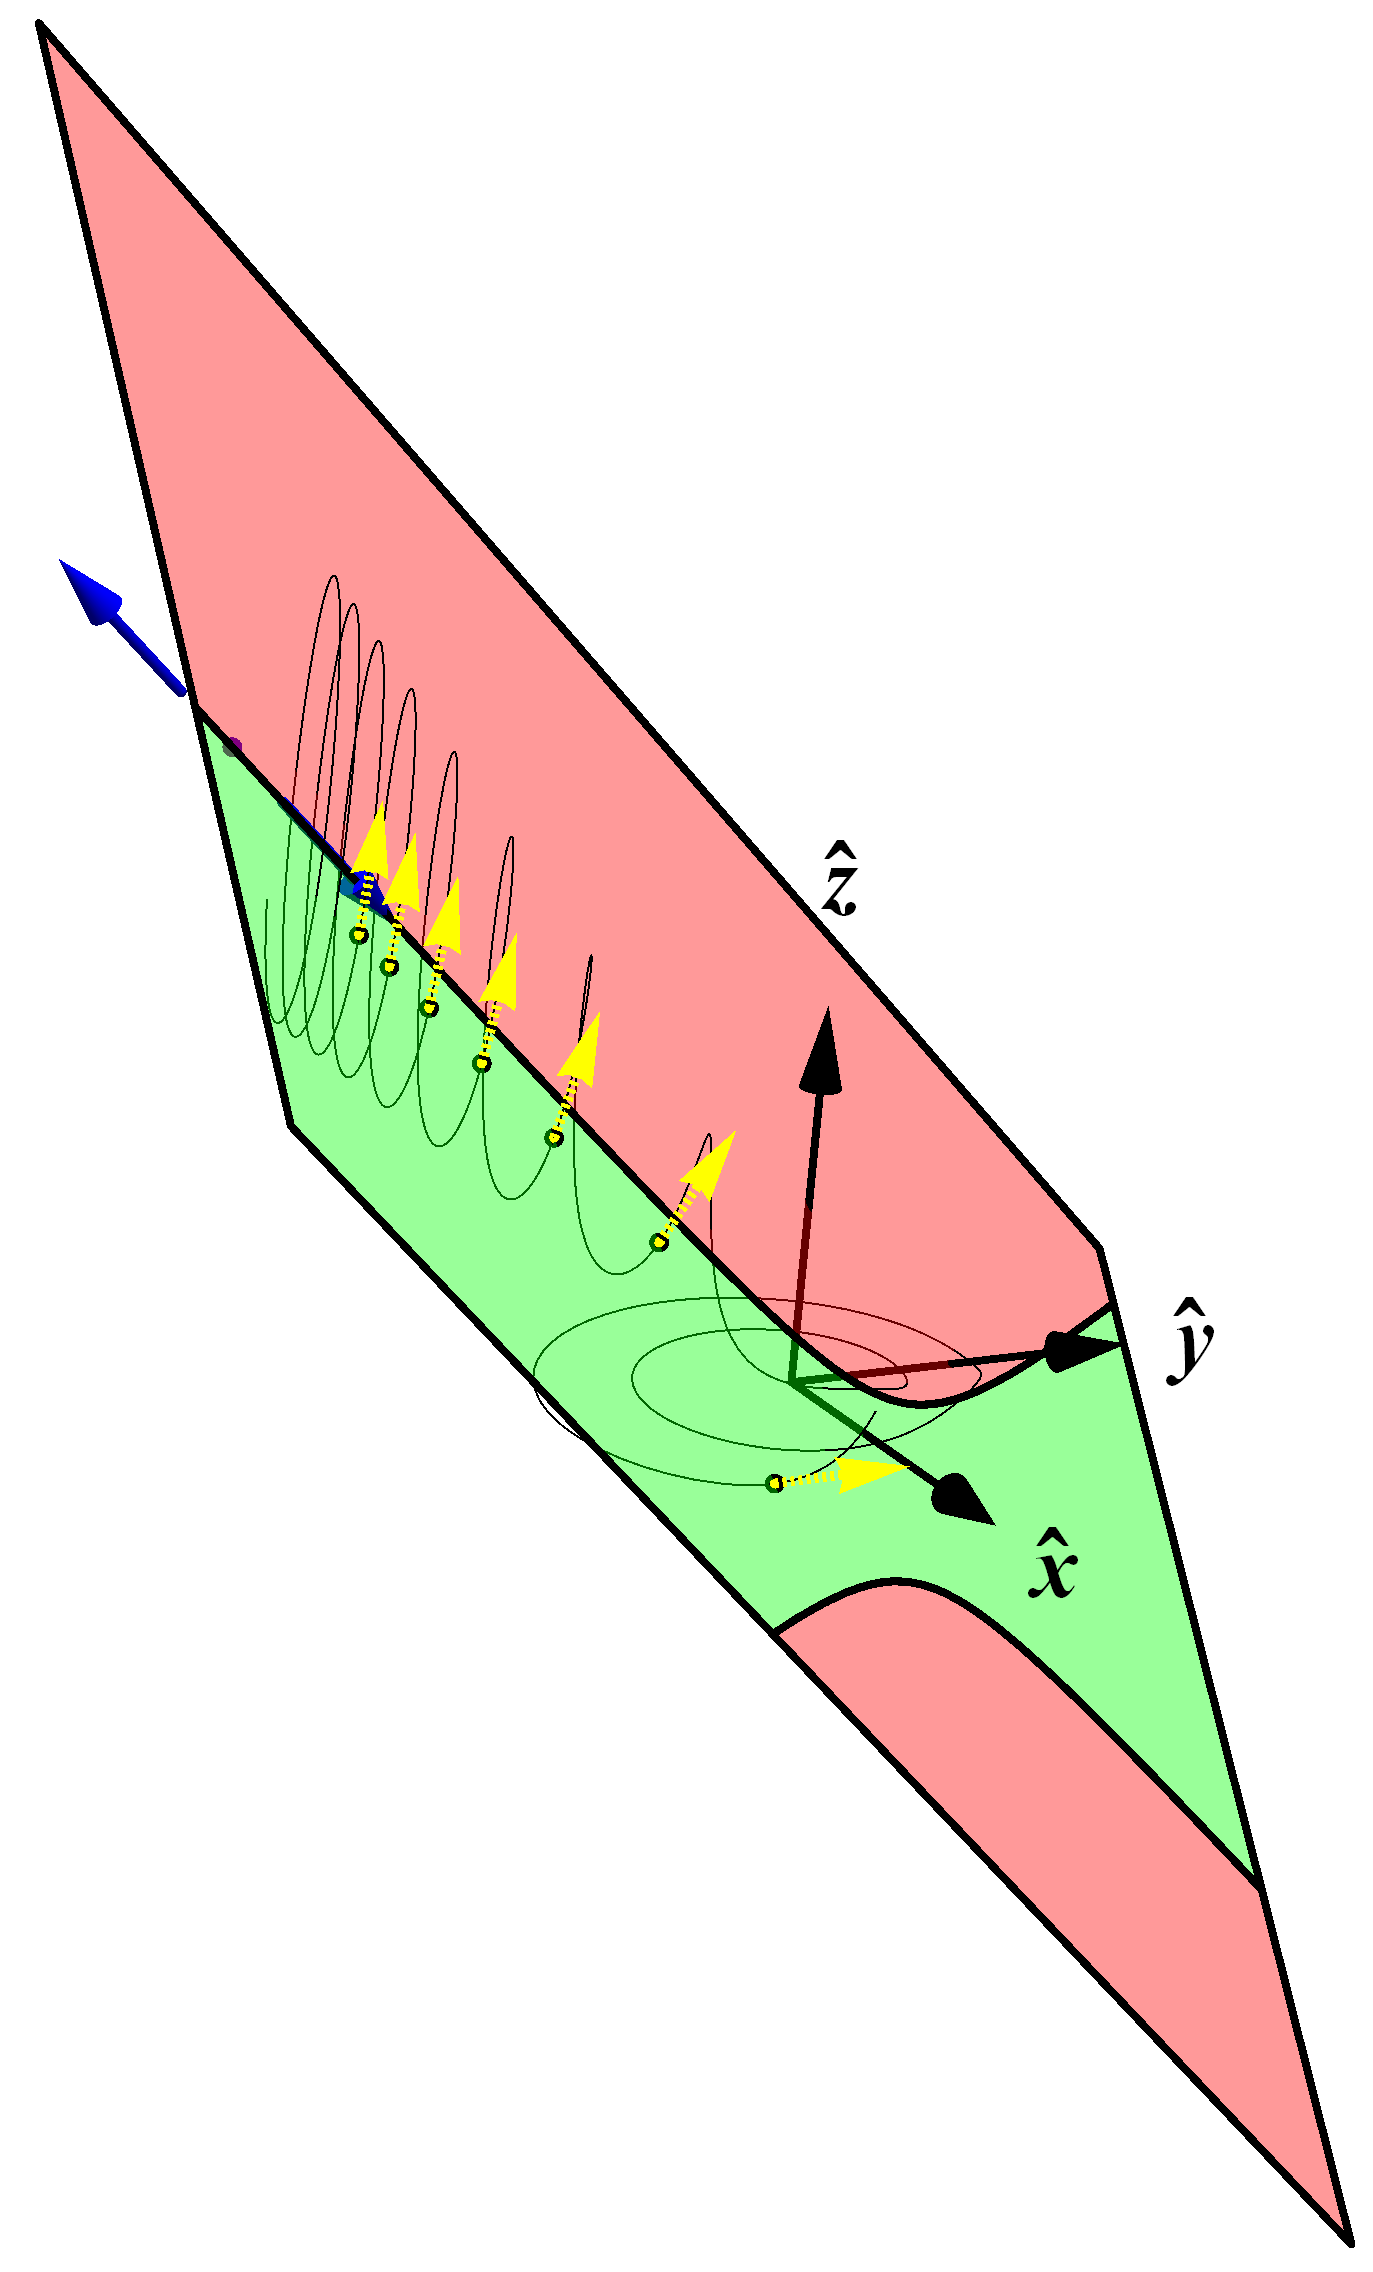
\includegraphics[width=0.19\textwidth,clip=true]{RoessFarEq3}%
(c)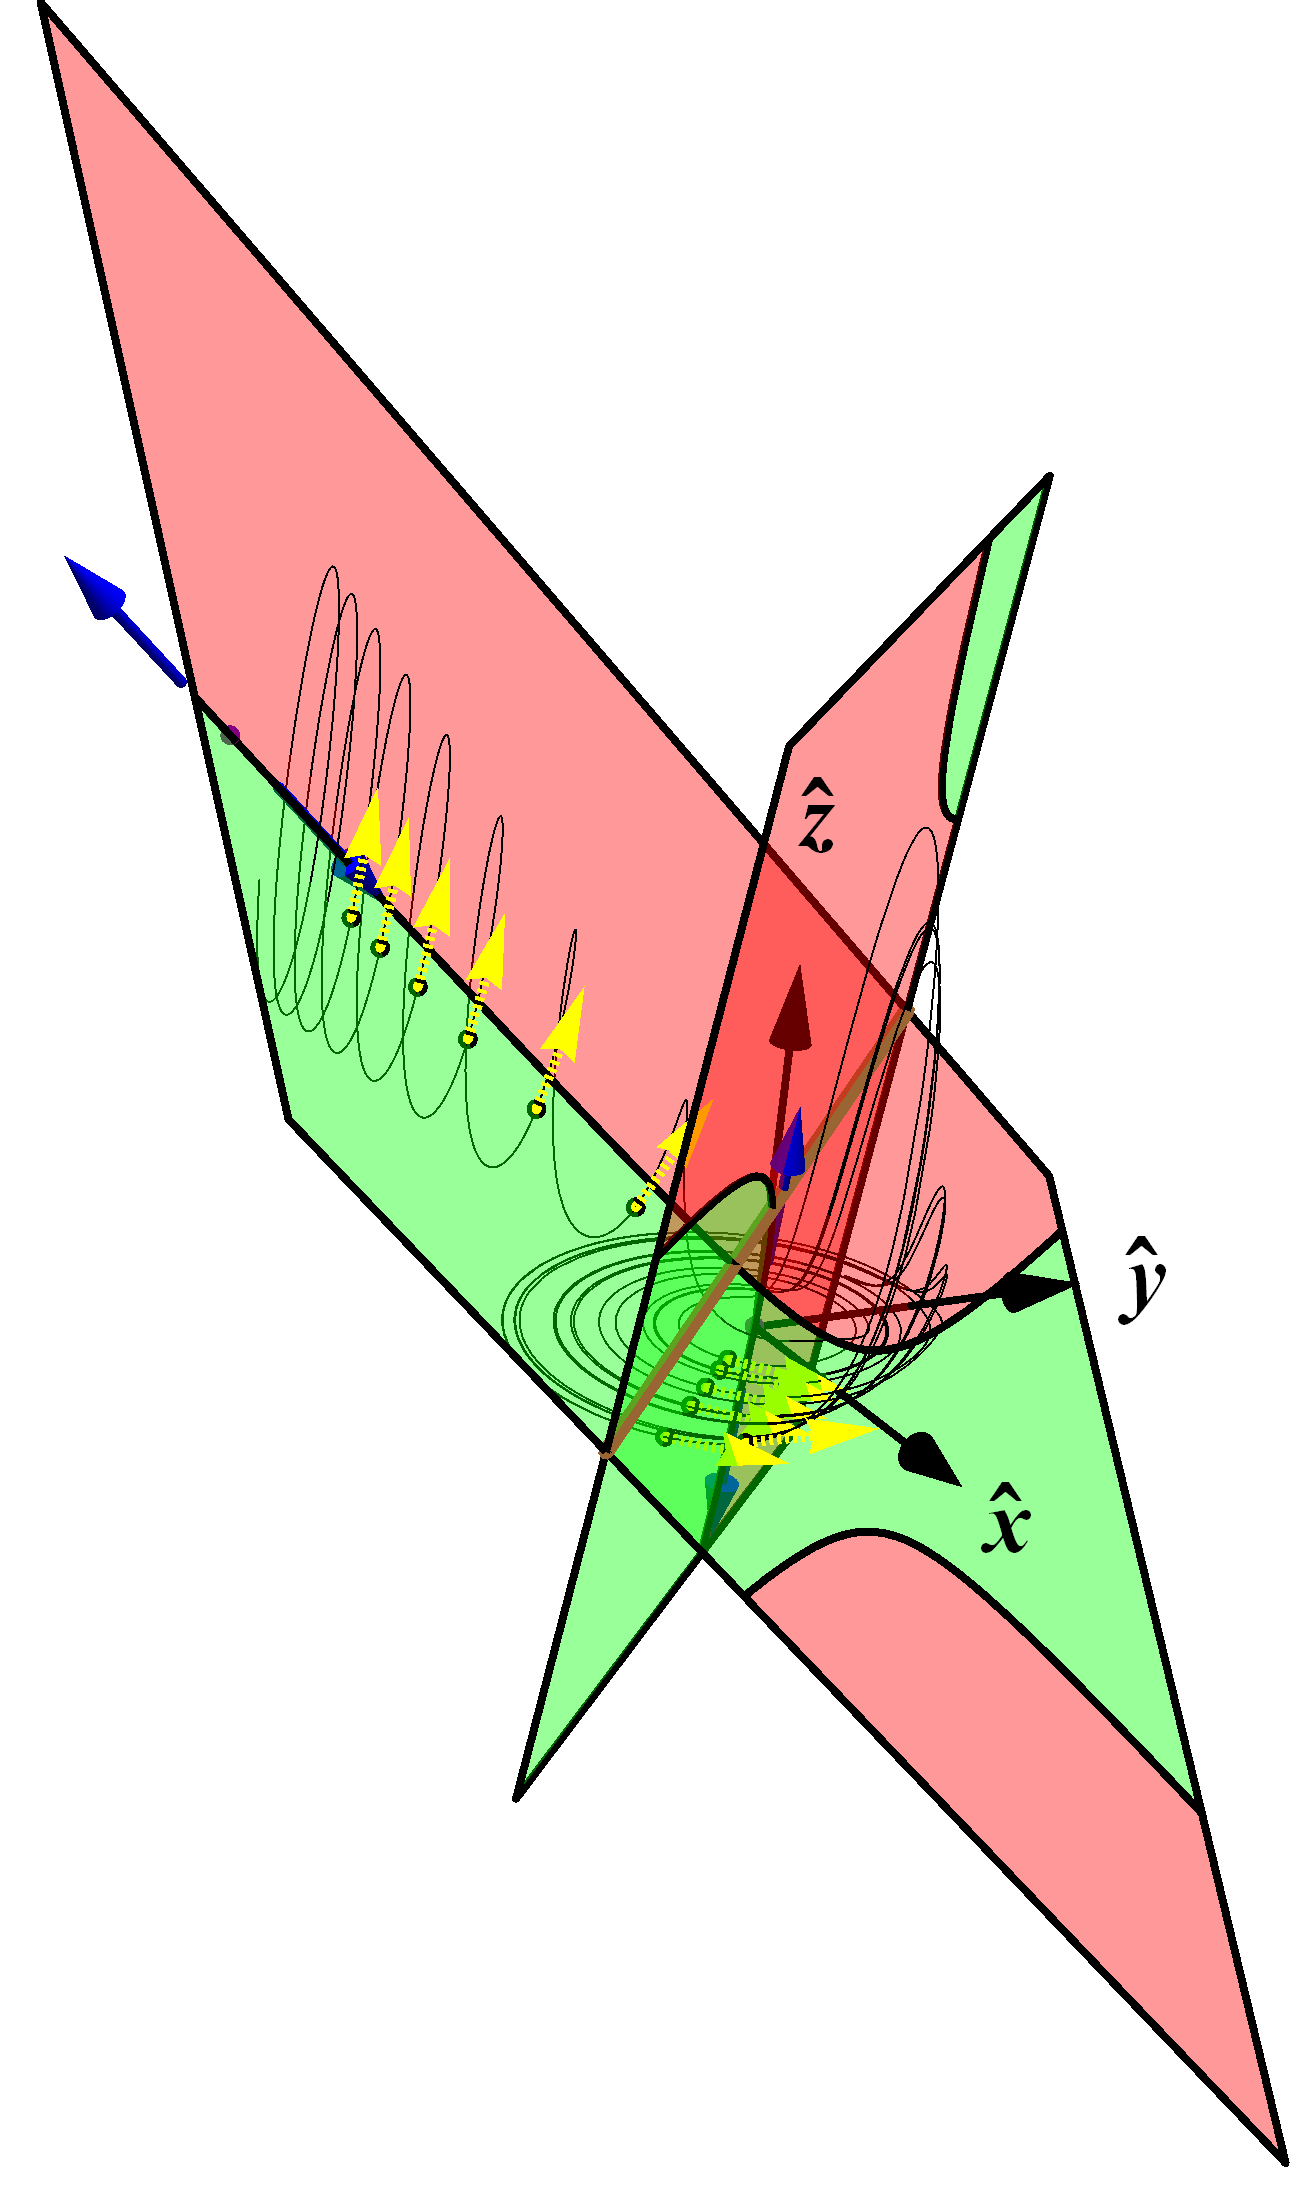
\includegraphics[width=0.27\textwidth,clip=true]{RoessSctAtlas3}
\end{center}
  \caption[R\"ossler section, outer {\eqv}]{
(a)
  A section through the outer {\eqv} $\slicep{}^{(+)}$  and its unstable
  eigenvector. The velocities $\vel(\sspRed_n)$ at the section crossings
  are indicated by yellow arrows. Note the ridge (brown line): the chart
  $\PoincS_{+}$ does not intersect the strange attractor.
(b)
  A two-chart atlas of R\"ossler flow, with charts $\PoincS_{-}$ and
  $\PoincS_{+}$ oriented and combined so that the ridge (intersection of
  the two sections, indicated by the brown line in the three figures)
  lies approximately between the \template s. The section hyperplanes
  beyond this ridge do not belong to the atlas.
  } \label{fig:RoessFarEq}
\end{figure}
%%%%%%%%%%%%%%%%%%%%%%%%%%%%%%%%%%%%%%%%%%%%%%%%%%%%%%%%%%%%%%%%%%%%%

For R\"ossler flow, the border condition \refeq{eq:sspRSing} yields a
quadratic condition in 3 dimensions, so the \poincBord s\ drawn in
\reffig{fig:RoessTrjs}\,(b) and \reffig{fig:RoessFarEq} are conic
sections. The two charts meet at a ridge, and together do a pretty good
job as the 2-chart atlas of the interesting R\"ossler dynamics. As
explained in ChaosBook.org,\rf{DasBuch} due to extreme contraction rate of
the attractor, the section in \reffig{fig:RoessTrjs}\,(b) is for all practical
purposes 1\dmn, and the associated return map yields all \po s of the 3\dmn\ flow.

In 3 dimensions everything -sections, ridges, \poincBord s- can be
drawn, and a chart does fit on a 2\dmn\ sheet of
papyrus. But what about for high-dimensional flows? The point of this
cartographical enterprise undertaken here is that while it is impossible to
visualize the 61,504% 61,506-2 $(d\!-\!2)$
\dmn\ {\poincBord} of the 61,505% 61,506-1 $(d\!-\!1)$
\dmn\ slab that is now our chart\rf{GibsonMovies}, a point is a point,
and a line is a line in a projection from any number of dimensions, so a
trajectory crossing of either a section or a {\poincBord} can be easily
determined and visualized in any dimension.

To summarize:
Evolution in time decomposes the \statesp\ into a spaghetti of 1\dmn\
trajectories $\ssp(\zeit)$, each determined by a single point $\ssp(0)$
on it. A well chosen set of \emph{sections} of codimension 1 allows us to
`quotient' the continuous time parameter $\zeit$, and reveal the
dynamically important transverse structure of flow's stable /unstable
manifolds. For unstable trajectories one needs, in addition, a notion of
recurrence to the section. The set of points $\{\sspRed_n\} =
\{\ssp(\zeit_n)\}$,  separated by short time section to section flights,
then captures the transverse dynamics without losing any information
about the chaotic flow. We can thus chart interesting regions of \statesp\ by
a picking a sufficient number of \template s and using them to construct charts
of their neighborhoods, each bounded by \poincBord s and ridges.

We close this section with two remarks on what sections \emph{are not}:

(1) A \PoincSec\ is {\em not} a projection onto a lower-dimensional
space. Rather, it is a local change of coordinates to a direction along
the flow $\vel(\sspRed)$, and the remaining coordinates transverse to it.
No information about the flow is lost; the full space trajectory
$\ssp(\zeit)$ can always be reconstructed by integration from its point
$\sspRed$ in the section.

(2) The method of \PoincSec s is {\em not} equivalent to \emph{strobing}
a flow at a sequence of instants in time. While `strobing' is what
numerical integrators and / or variational methods\rf{lanVar1} do, by
representing a trajectory as a sequence of points separated by time-integration
steps, it does not reduce the flow to a codimension 1 manifold, as the
sequence of strobed points still resides in the full $d$-dimensional \statesp.


\section{Dancers and drifters}
% and symmetries}
% Dynamics and symmetry
\label{s:symm}

%% A27*-pipeSymms.* - read dasbuch/book/FigSrc/inkscape/00ReadMe.txt
 \begin{figure}
 \begin{center}
  \setlength{\unitlength}{0.20\textwidth}
  %% \unitlength = units used in the Picture Environment
(a)
  \begin{picture}(1,0.52454249)%
    \put(0,0){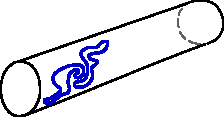
\includegraphics[width=\unitlength]{A27a-pipeSymms}}%
    \put(0.61583231,0.13683004){\color[rgb]{0,0,0}\makebox(0,0)[lb]{\smash{$z$}}}%
    \put(0.00611823,0.27217453){\color[rgb]{0,0,0}\makebox(0,0)[lb]{\smash{$\theta$}}}%
  \end{picture}%
(b)
  \begin{picture}(1,0.52454249)%
    \put(0,0){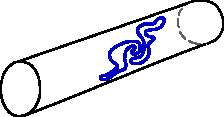
\includegraphics[width=\unitlength]{A27b-pipeSymms}}%
    \put(0.61583231,0.13683004){\color[rgb]{0,0,0}\makebox(0,0)[lb]{\smash{$z$}}}%
    \put(0.00611823,0.27217453){\color[rgb]{0,0,0}\makebox(0,0)[lb]{\smash{$\theta$}}}%
  \end{picture}%
\\
(c)
  \begin{picture}(1,0.52454249)%
    \put(0,0){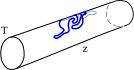
\includegraphics[width=\unitlength]{A27c-pipeSymms}}%
    \put(0.61583231,0.13683004){\color[rgb]{0,0,0}\makebox(0,0)[lb]{\smash{$z$}}}%
    \put(0.00611823,0.27217453){\color[rgb]{0,0,0}\makebox(0,0)[lb]{\smash{$\theta$}}}%
  \end{picture}%
(d)
  \begin{picture}(1,0.52454249)%
    \put(0,0){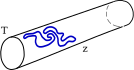
\includegraphics[width=\unitlength]{A27d-pipeSymms}}%
    \put(0.61583231,0.13683004){\color[rgb]{0,0,0}\makebox(0,0)[lb]{\smash{$z$}}}%
    \put(0.00611823,0.27217453){\color[rgb]{0,0,0}\makebox(0,0)[lb]{\smash{$\theta$}}}%
  \end{picture}%
 \end{center}
 \caption[$\On{2}_\theta \times \SOn{2}_z$ symmetry of flow in a stream-wise
          periodic pipe]{
A fluid state in a pipe translated or rotated is
also a solution. In particular, a \rpo\ $\pS_p$ is
(a) a \emph{time dependent} state of the fluid that after a period $\period{p}$ reemerges
(b) translated by downstream shift $\shift_p$
(such solutions are $\SOn{2}_z$ equivariant in a stream-wise periodic pipe),
(c) translated by downstream shift $\shift_p$ and rotated azimuthally by $\gSpace_p$
(i.e., $\SOn{2}_{\phi} \times \SOn{2}_z$ equivariant) or,
(d) reflected and rotated azimuthally by $\gSpace$ (i.e., $\On{2}_{\phi}$ equivariant).
Consider this in contrast to a \reqv, a constant shape that travels
downstream with constant {\phaseVel} $\velRel$. (from \wwwcb{})
 }\label{fig:A27-pipeSymms}
 \end{figure}
%% A27*-pipeSymms.* %%%%%%%%%%%%%%%%%%%%%%%%%%%%%%%%%%%%%%%%%%%%%%%%%%%%%%%

What is a symmetry? A visualization of the fluid dynamics of a pipe flow,
\reffig{fig:A27-pipeSymms}, affords an intuitive illustration. Solutions
of pipe flow remain physically the same under azimuthal rotations and
stream-wise translations (which become \SOn{2} rotations in numerical
stream-wise periodic pipes) but correspond to different points in
\statesp\ and may look very different in visualizations.

Each \SOn{2} group orbit is topologically a circle, but it traces out a
complicated \statesp\ curve composed of many Fourier modes that are nonlinearly
coupled and thus of comparable magnitude. Together,
the two \SOn{2} rotations sweep out contorted and hard to visualize $T^2$ tori (see
\refref{ACHKW11}), so here we shall illustrate the key ideas by a much
simpler example, the $\SOn{2}$-equivariant Gibbon and
McGuinness\rf{GibMcCLE82,FowlerCLE82} \cLe\ of geophysics and laser
physics,
\bea
	\dot{x}_1 &=& -\sigma x_1 + \sigma y_1
        \,,\qquad
	\dot{x}_2 \,=\, -\sigma x_2 + \sigma y_2
        \continue
	\dot{y}_1 &=& (\RerCLor-z) x_1 - \ImrCLor x_2 -y_1-e y_2 \continue
	\dot{y}_2 &=& \ImrCLor x_1 + (\RerCLor-z) x_2 + e y_1- y_2\continue
	\dot{z} \; &=& -b z + x_1 y_1 + x_2 y_2
    \,.
\label{eq:CLeR}
\eea
Here, the parameters are set to Siminos's values\rf{SiminosThesis} $\RerCLor=28,\,
\ImrCLor=0,\, b=8/3,\, \sigma=10,\, e= 1/10$.
For a review of the historical background and an in-depth investigation of the model see \refrefs{SiminosThesis,SiCvi10}.

\begin{figure}
  	\begin{center}
  	\setlength{\unitlength}{0.20\textwidth}
  (a)
  	\begin{picture}(1,1.07802818)%
    	\put(0,0){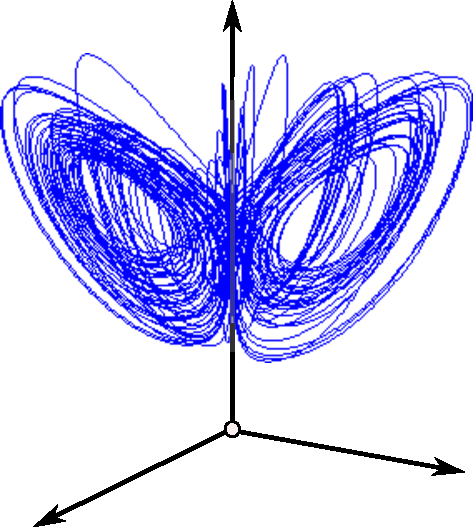
\includegraphics[width=\unitlength]{CLEattractor}}%
    	\put(0.55152995,1.0139628){\color[rgb]{0,0,0}\makebox(0,0)[lb]{\smash{$z$}}}%
    	\put(0.05573445,0.0739776){\color[rgb]{0,0,0}\makebox(0,0)[lb]{\smash{$x_1$}}}%
    	\put(0.90013492,0.16491708){\color[rgb]{0,0,0}\makebox(0,0)[lb]{\smash{$x_2$}}}%
  	\end{picture}%	
  (b)
  	\begin{picture}(1,1.06440474)%
    	\put(0,0){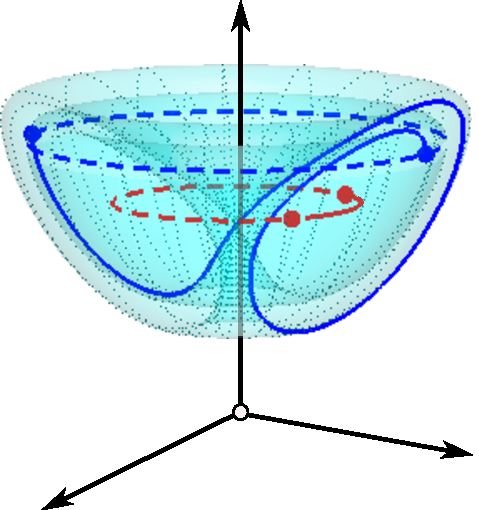
\includegraphics[width=\unitlength]{CLEWurst01}}%
   		\put(0.55961552,1.00214901){\color[rgb]{0,0,0}\makebox(0,0)[lb]{\smash{$z$}}}%
   		\put(0.07008555,0.07304272){\color[rgb]{0,0,0}\makebox(0,0)[lb]{\smash{$x_1$}}}%
    	\put(0.90381504,0.16283301){\color[rgb]{0,0,0}\makebox(0,0)[lb]{\smash{$x_2$}}}%
  	\end{picture}	
    \end{center}
  \caption
  [\CLf: $\cycle{01}$ {\rpo} group orbit]{
  (a)
  The strange attractor of \cLf.
  (b)
  The initial \reqv\ $\REQV{}{1}$ point is shown by the red dot, and its
  group orbit / trajectory by the dashed red line. One period of the
  $\cycle{01}$ {\rpo} is shown by the solid blue line. The group orbit of
  its (arbitrary) starting point is shown by the dashed blue line: after
  one period the trajectory has returned to the group orbit but with a
  different phase. The \wurst, \ie, the group orbit of the $\cycle{01}$
  trajectory (dark blue) is shown by the cyan surface. Trajectory of the
  further 15 repeats of $\cycle{01}$ (faint dotted lines) traces out this
  torus; in that time the slowly drifting \reqv\ $\REQV{}{1}$ has
  advanced to the next red dot (red line).
  }
\label{fig:CLf01group}
\end{figure}

The strange attractor of the \cLf\ \reffig{fig:CLf01group}\,(a), in its
present state, is a complete mess. Because of the continuous symmetry, solutions tend to drift along rather
than dance to distant neighborhoods, with the physically important
shape-changing dynamics hidden from view. Yet embedded within the
strange attractor lies a multitude of dynamically important trajectories.

In the complex Lorenz system, we find an example of the ultimate drifter,
a signature invariant solution that signals presence of a continuous symmetry; A {\em \reqv} (traveling wave,
rotational wave, ...) is a trajectory whose velocity field lies within
the group tangent space, such that
\(
\vel(\ssp) = c \cdot \groupTan(\ssp)
\) %\label{phaseVel}
with a constant {\phaseVel} $c$, and whose time evolution is thus
confined to the group orbit (see \reffig{fig:CLf01group}\,(b)); think of an unchanging body carried by a
stream.

A {\em \rpo} behaves more like a dancer. $\pS_p$ is a trajectory that
recurs exactly
\beq
\ssp(\zeit) = \LieEl_p \, \ssp(\zeit + \period{p} )
    \,,\qquad
\ssp(\zeit) \in \pS_p
\ee{RPOrelper1}
after a fixed {relative period} $\period{p}$, but shifted by a fixed
group action ${\LieEl_p}$ that maps the endpoint $\ssp (\period{p}) $ back
into the initial point cycle point $\ssp (0) $; think of a dancer moving
across the stage through a set of motions and then striking the initial
pose,\rf{ShWi06} or study the pipe flow sketches in \reffig{fig:A27-pipeSymms}.

Because the $\SOn{2}$ transformations act on the \cLf\ only through the
simplest, $m=1$ Fourier mode, here all group orbits are circles, and appear
elliptical in most $d=5 \to 3$~dimensions projections. Nevertheless, even
the \wurst\ traced out by the very simplest, short \rpo\ $\cycle{01}$\rf{SiCvi10} shown
in \reffig{fig:CLf01group}\,(b) is not so easy to get one's head around:
you are looking at a 3\dmn\ projection of a \emph{torus} embedded in 5
dimensions.

%%%%%%%%%%%%%%%%%%%%%%%%%%%%%%%%%%%%%%%%%%%%%%%%%
% 2011-09-09, 2012-03-30 Predrag: add BeThMovFr to
%            continuous.tex overheads, and ChaosBook
% replace A27movFrame*.* everywhere
\begin{figure}
 \begin{center}
  \setlength{\unitlength}{0.20\textwidth}
  %% \unitlength = units used in the Picture Environment
(a)~~
  \begin{picture}(1,0.98655417)%
    \put(0,0){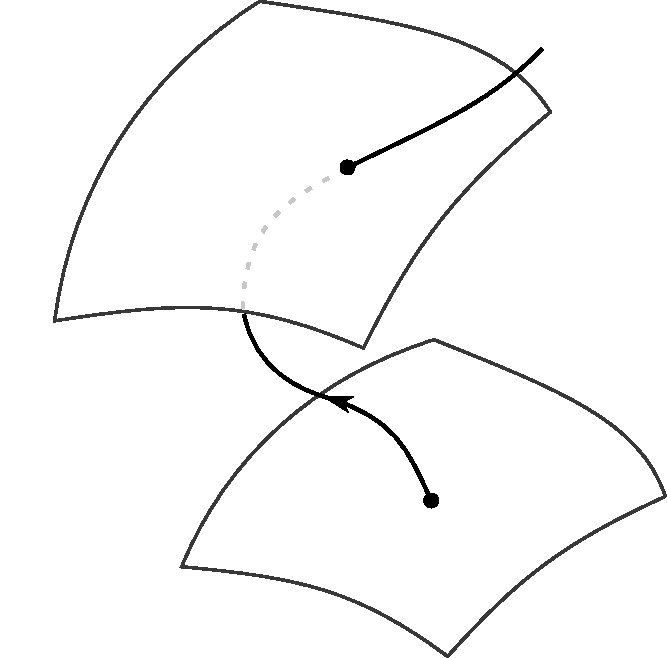
\includegraphics[width=\unitlength]{BeThTrajTeX}}%
    \put(0.35976094,0.91875614){\color[rgb]{0,0,0}\rotatebox{-16.32889204}{\makebox(0,0)[lb]{\smash{$\pS_{\ssp(\zeit)}$}}}}%
        \put(0.60333631,0.42274457){\color[rgb]{0,0,0}\rotatebox{-30.8073288}{\makebox(0,0)[lb]{\smash{$\pS_{\ssp(0)}$}}}}%
    \put(0.63001383,0.14959019){\color[rgb]{0,0,0}\rotatebox{0.0313674}{\makebox(0,0)[lb]{\smash{$\ssp(0)$}}}}%
    \put(0.4558276,0.64524238){\color[rgb]{0,0,0}\rotatebox{0.0313674}{\makebox(0,0)[lb]{\smash{$\ssp(\zeit)$}}}}%
    \put(0.13110825,0.05766516){\color[rgb]{0,0,0}\rotatebox{0.11031334}{\makebox(0,0)[lb]{\smash{$\pS$}}}}%
  \end{picture}%
~~(b)
  \begin{picture}(1,0.98742208)%
    \put(0,0){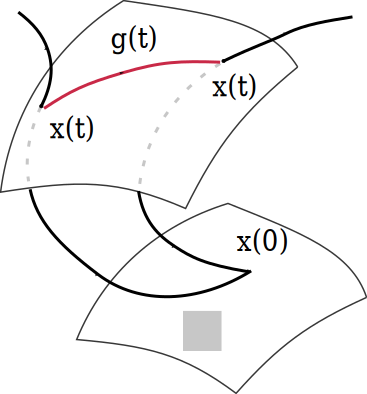
\includegraphics[width=\unitlength]{BeThMovFr}}%
    \put(0.20546387,0.64069775){\color[rgb]{0,0,0}\rotatebox{0.0313674}{\makebox(0,0)[lb]{\smash{$\ssp(\zeit)$}}}}%
    \put(0.7334028,0.27844745){\color[rgb]{0,0,0}\rotatebox{0.0313674}{\makebox(0,0)[lb]{\smash{$\sspRed(0)$}}}}%
    \put(0.52082757,0.7302884){\color[rgb]{0,0,0}\rotatebox{0.0313674}{\makebox(0,0)[lb]{\smash{$\sspRed(\zeit)$}}}}%
    \put(0.35738205,0.88152375){\color[rgb]{0,0,0}\rotatebox{0.0313674}{\makebox(0,0)[lb]{\smash{$\LieEl(\zeit)$}}}}%
    \put(0.48490227,0.11640486){\color[rgb]{0,0,0}\rotatebox{0.0313674}{\makebox(0,0)[lb]{\smash{$\ssp(0)$}}}}%
    \put(0.3947908,0.25892637){\color[rgb]{0,0,0}\rotatebox{0.0313674}{\makebox(0,0)[lb]{\smash{$\LieEl(0)$}}}}%
  \end{picture}%
 \end{center}
  \caption{\label{fig:BeThMovFr}
(a)
The group orbit $\pS_{\ssp(0)}$ of \statesp\ point $\ssp(0)$, and the
group orbit $\pS_{\ssp(\zeit)}$ reached by the trajectory $\ssp(\zeit)$ a time $\zeit$
later.
(b)
Two physically equivalent trajectories $\ssp(\zeit)$ and $\sspRed(\zeit)$
are related, in general, by an arbitrary, time dependent {\em moving frame} transformation $\LieEl(\zeit)$, such that $\ssp(\zeit)=\LieEl(\zeit)\,\sspRed(\zeit)$ (from \wwwcb{}).
  }
\end{figure}
%%%%%%%%%%%%%%%%%%%%%%%%%%%%%%%%%%%%%%%%%%%%%%%%%%

To summarize: continuous symmetries in the dynamics stratify the \statesp\
into an onion, where each layer is a group orbit (\reffig{fig:BeThMovFr}). How are we to sort out this mess? Luckily, all the points on a group orbit are physically equivalent, so we are
free to replace a given flow $\ssp(\zeit)$ by another \sspRed(\zeit), such that $\ssp(\zeit)=\LieEl(\zeit)\,\sspRed(\zeit)$ for any (in general, time dependent) {\em moving frame}\rf{FelsOlver98,FelsOlver99,OlverInv} transformation $\LieEl(\zeit)$. For example, to film our dancer, we can mount the camera
on a cart moving alongside her. So, in the presence of continuous symmetries,
there are two kinds of motion: those of a dancer, continuously changing
shapes, and those of a drifter, merely shuffling along the easy, shape invariant directions. We will presently banish the drifters, and just enjoy the dance.

%%%%%%%%%%%%%%%%%%%%%%%%%%%%%%%%%%%%%%%%%%%%%%%%%%%%%%%%%%%%%%%%
 %% chartBord-m*.* replaces FrCv11.tex inflectHype.*
 \begin{figure}
 \begin{center}
  \setlength{\unitlength}{0.20\textwidth}
  %% \unitlength = units used in the Picture Environment
(a)
  \begin{picture}(1,0.91596465)%
    \put(0,0){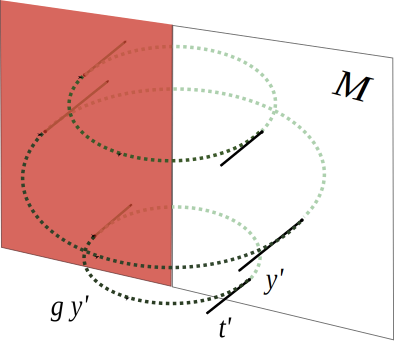
\includegraphics[width=\unitlength]{chartBord-m1}}%
    \put(0.84045332,0.62950567){\color[rgb]{0,0,0}\makebox(0,0)[lb]{\smash{$\pSRed$}}}%
    \put(0.08835189,0.14720037){\color[rgb]{0,0,0}\makebox(0,0)[lb]{\smash{$\LieEl\slicep$}}}%
    \put(0.67299795,0.18547195){\color[rgb]{0,0,0}\makebox(0,0)[lb]{\smash{$\slicep$}}}%
    \put(0.44341875,0.03071734){\color[rgb]{0,0,0}\makebox(0,0)[lb]{\smash{$\sliceTan{}$}}}%
  \end{picture}%
\\
(b)
  \begin{picture}(1,0.91727402)%
    \put(0,0){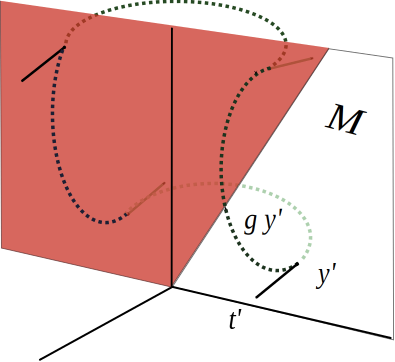
\includegraphics[width=\unitlength]{chartBord-m2}}%
    \put(0.82257887,0.59549577){\color[rgb]{0,0,0}\makebox(0,0)[lb]{\smash{$\pSRed$}}}%
    \put(0.80526889,0.1997715){\color[rgb]{0,0,0}\makebox(0,0)[lb]{\smash{$\slicep$}}}%
    \put(0.55844296,0.0631667){\color[rgb]{0,0,0}\makebox(0,0)[lb]{\smash{$\sliceTan{}$}}}%
    \put(0.61811177,0.33705605){\color[rgb]{0,0,0}\makebox(0,0)[lb]{\smash{$\LieEl\slicep$}}}%
  \end{picture}%
 \end{center}
 \caption{\label{fig:chartBord}  %fig:slice}
The \chartBord\ ${\cal}$ is the $(d\!-\!2)$\dmn\ hyperplane that contains
all the points $\sspRSing$ whose group tangents $\groupTan(\sspRSing)$
lie in the \slice\ hyperplane or vanish and are thus normal to
$\sliceTan{}$. Beyond this boundary, the group orbits pierce the \slice\
hyperplane in the wrong direction, so \emph{only} the half-hyperplane
that contains the \template\ belongs to the slice. The {\chartBord} is
not easy to visualize; For the lack of dimensions, here it is drawn as a
`line,' the $z$ axis in this 3\dmn\ sketch. (a) If the equivariant
coordinates transform only under the $m=1$ representation of $\SOn{2}$,
every group orbit is a circle, and crosses any slice hyperplane exactly
twice. However, if there are coordinates that transform as higher $m$,
the group orbit can pierce the hyperplane up to $2m$ times, and the
{\chartBord} lies closer to the template:  For example, (b) a group orbit
for a combination of $m=1$ and $m=2$ equivariant coordinates resembles
the seam of a baseball, and can cross the \emph{slice hyperplane} 4 times,
out of which only the point closest to the \template\ is in the
\emph{slice} (from \wwwcb{}).
 }%
 \end{figure}
%%%%%%%%%%%%%%%%%%%%%%%%%%%%%%%%%%%%%%%%%%%%%%%%%%%%%%%%%%%%%%%%

\section{Chart}
\label{s:slice}

Suppose your day job is computing invariant solutions of the \NSe. Do you
really want to compute the same solution over and over again, for every
point on the group orbit? No, you would like to compute it only once. The
strategy for picking out that one representative solution is called \emph{symmetry
reduction}. Its goal is to replace each group orbit by a unique point in
a lower-dimensional symmetry-\reducedsp\ $\pSRed \subset \pS/\Group$, as
sketched in \reffig{fig:BeThTraj}.

%%%%%%%%%%%%%%%%%%%%%%%%%%%%%%%%%%%%%%%%%%%%%%%%%
% 2011-08-23 Predrag: replaces BeThTraj.pdf from
% dasbuch/book/FigSrc/inkscape/BeThTraj.svg
% 2011-09-09 Predrag: updated
%            continuous.tex overheads, and ChaosBook
\begin{figure}
 \begin{center}
  \setlength{\unitlength}{0.20\textwidth}
  %% \unitlength = units used in the Picture Environment
(a)~~
  \begin{picture}(1,0.98655417)%
    \put(0,0){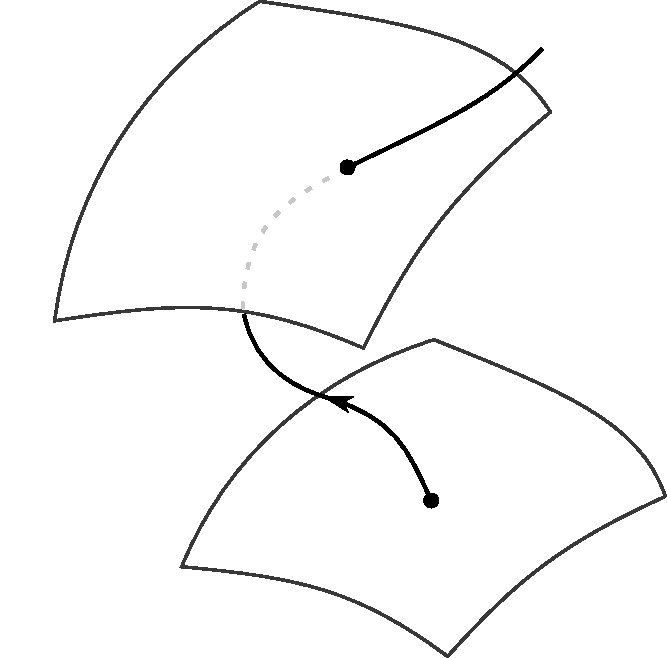
\includegraphics[width=\unitlength]{BeThTrajTeX}}%
    \put(0.35976094,0.89875614){\color[rgb]{0,0,0}\rotatebox{-10.32889204}{\makebox(0,0)[lb]{\smash{$\pS_{\ssp(\zeit)}$}}}}%
    \put(0.59333631,0.39274457){\color[rgb]{0,0,0}\rotatebox{-20.8073288}{\makebox(0,0)[lb]{\smash{$\pS_{\ssp(0)}$}}}}%
    \put(0.66001383,0.16959019){\color[rgb]{0,0,0}\rotatebox{0.0313674}{\makebox(0,0)[lb]{\smash{$\ssp(0)$}}}}%
    \put(0.4658276,0.64524238){\color[rgb]{0,0,0}\rotatebox{0.0313674}{\makebox(0,0)[lb]{\smash{$\ssp(\zeit)$}}}}%
    \put(0.13110825,0.05766516){\color[rgb]{0,0,0}\rotatebox{0.11031334}{\makebox(0,0)[lb]{\smash{$\pS$}}}}%
  \end{picture}%
~~(b)
  \begin{picture}(1,1.07315413)%
    \put(0,0){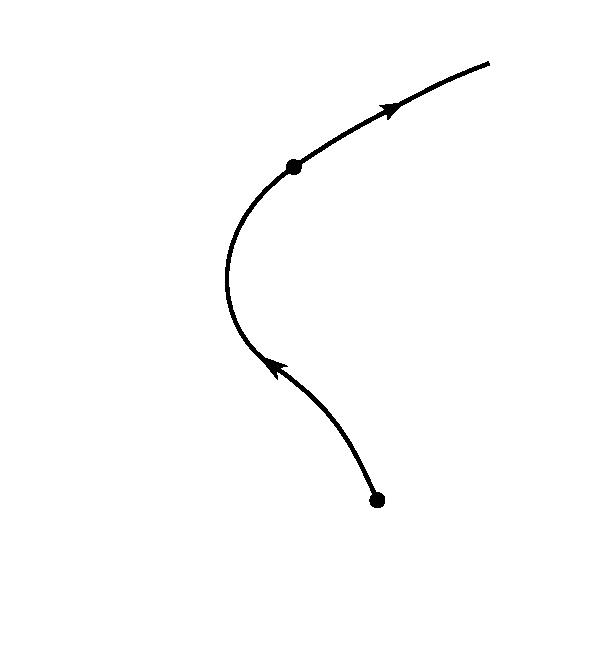
\includegraphics[width=\unitlength]{BeThRedTeX}}%
    \put(0.19912369,0.17144733){\color[rgb]{0,0,0}\rotatebox{0.11031334}{\makebox(0,0)[lb]{\smash{$\pSRed$}}}}%
    \put(0.63028127,0.18433598){\color[rgb]{0,0,0}\rotatebox{0.03136739}{\makebox(0,0)[lb]{\smash{$\sspRed(0)$}}}}%
    \put(0.48253394,0.69182305){\color[rgb]{0,0,0}\rotatebox{0.03136739}{\makebox(0,0)[lb]{\smash{$\sspRed(\zeit)$}}}}%
  \end{picture}%
 \end{center}
% (a) 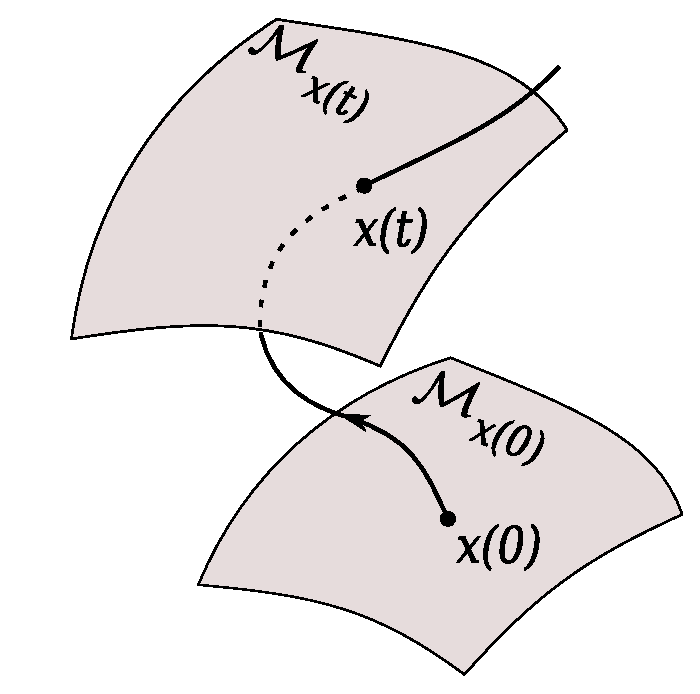
\includegraphics[width=0.45\textwidth]{BeThTraj}
  \caption{\label{fig:BeThTraj} (a) The group orbit $\pS_{\ssp(0)}$ of \statesp\ point $\ssp(0)$, and the
group orbit $\pS_{\ssp(\zeit)}$ reached by the trajectory $\ssp(\zeit)$ time $t$
later.
(b) Symmetry reduction $\pS \to \pSRed$ replaces $\pS_{\ssp}\subset\pS$ by a
single point $\sspRed \in \pSRed$.
  }
\end{figure}
%%%%%%%%%%%%%%%%%%%%%%%%%%%%%%%%%%%%%%%%%%%%%%%%%%

What is a smart way to go about it? Intuition gained from pipe flow (see
\reffig{fig:A27-pipeSymms}), will again prove helpful. A turbulent flow
exhibits a myriad of unstable structures, all traveling down the pipe
with its own {\phaseVel}. The
\mslices\rf{rowley_reconstruction_2000,BeTh04,SiCvi10,FrCv11} that we now
describe tells you how to pull each solution back into a {\em fixed}
frame called a \emph{\slice} and compare it to your repertoire of
precomputed solutions, or the \template s $\{\slicep{}^{(j)}\}$, using
the principle of the closest distance to each. What follows is very much
like the construction of sections of \refsect{s:cut}; due to the linear
action of the symmetry group, slicing is easier than sectioning, but
wholly unfamiliar. This is why we warmed up by reviewing the \PoincSec s.
We now offer a pictorial tour of this
(save for the one bold incursion\rf{ACHKW11})
hitherto uncharted territory.
    \PC{to Daniel - if you do not use footnotes but embed the editorials
    into the text proper, they do not get turned off when we turn the
    draft switch off - dangerous practice, as if you again make me submit
    the paper at 2AM some of these private doubts will go straight to the
    readers and referees - so I am now again stuck in Howey 9:15PM - no,
    already 10:30PM - with the Memphis blues again, making them into
    footnotes while I would much rather bicycle home and ...zzz...}
    \DB{2012-04-19}{Obviously other people have looked at the method of
    slices... we cite them!
    \\{\bf Predrag} I wish you were right, because then we would not have
    to write yet another paper on slices. This is not a paper about
    single slice hyperplane, it is about how you construct an atlas over
    a slice of interest. \refRefs{rowley_reconstruction_2000,BeTh04} only
    study \reqva\ of PDEs, and for that a single slice hyperplane
    suffices, they do not mention anything about \chartBord s - if you
    find them anyplace in literature, please alert me. Ditto for
    \poincBord s, I have never seen them defined anywhere.
    \refRef{SiCvi10} is about \cLe, and notices that there is a
    \chartBord\ (calls it `singularity set') but waffles about it, as it
    has no notion of distance and a chart. \refRef{FrCv11} uses the
    notion of the closest distance first noted in
    \refref{rowley_reconstruction_2000} to define a neighborhood and
    explain the jump induced by \chartBord\ crossing. We tried and failed
    to construct a two-chart for \cLe. \refRef{ACHKW11} is the first and
    still only attempt at implementation of the atlas idea - I fear
    Ashley is in error as long as \reffig{fig:A29-2tmplts}\,(b) is not
    implemented, that is why we never found any \rpo s beyond the lower
    edge of turbulence. But I do not think adding all this info to the
    paper aids the reader one iotta, it only makes the paper longer. I
    can stick all this into remarks in ChaosBook.org, but it's beyond
    point here.
    }
First, pick a \template\ $\slicep$ and use the freedom to shift and
rotate it (\reffig{fig:BeThMovFr}\,(b)) until it overlies, as well as
possible, the state $\ssp$, by minimizing the distance
\beq
\Norm{\ssp - \LieEl(\gSpace)\,\slicep}
\, .
\ee{minDistance}
Now, replace the entire group orbit of $\ssp$ by the closest match to the
template pattern, given by $\sspRed=\LieEl^{-1}\ssp$. The
symmetry-\reducedsp\ $\pSRed$ is comprised of such closest matches, a
point for each full \statesp\ group orbit. From here on, we will use the
hat on $\sspRed$ to indicate the unique point on the group orbit of
$\ssp$ that is closest to the \template\ \slicep.
    \PC{Daniel left these two symbols: ``
$\pS$
\ssp
    '' floating freely here, do not know why?
    }

%%%%%%%%%%%%%%%%%%%%%%%%%%%%%%%%%%%%%%%%%%%%%%%%%%%%%%%%%%%%%%%%%%%%%
\begin{figure}
	\begin{center}
  	\setlength{\unitlength}{0.25\textwidth}
  	\begin{picture}(1,0.62007592)%
    	\put(0,0){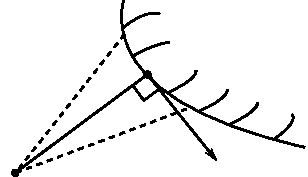
\includegraphics[width=\unitlength]{A28extremum2}}%
    	\put(0.8274739,0.27313042){\color[rgb]{0,0,0}\makebox(0,0)[lb]{\smash{$\pS_{\slicep}$}}}%
    	\put(0.71822871,0.05712263){\color[rgb]{0,0,0}\makebox(0,0)[lb]{\smash{$\sliceTan{}$}}}%
    	\put(-0.00055527,0.03229441){\color[rgb]{0,0,0}\makebox(0,0)[lb]{\smash{$\sspRed$}}}%
    	\put(0.50966967,0.34820145){\color[rgb]{0,0,0}\makebox(0,0)[lb]{\smash{$\slicep$}}}%
  	\end{picture}
  \end{center}
  \caption{\label{fig:A28extremum}
  Extremal condition \refeq{PCsectQ0} for the point $\sspRed$ on the
  $\ssp$ group orbit that is nearest to the \template\ $\slicep$.
  }
\end{figure}
%%%%%%%%%%%%%%%%%%%%%%%%%%%%%%%%%%%%%%%%%%%%%%%%%%%%%%%%%%%%%%%%%%%%%


The minimal distance satisfies
the extremum condition (\reffig{fig:A28extremum})
\[
\frac{\partial}{\partial \gSpace} \Norm{\ssp - \LieEl(\gSpace)\,\slicep}^2
   =
2\, \braket{\sspRed - \slicep}{\sliceTan{}}
   = 0
        \,,\quad
\sliceTan{} = \Lg \slicep
\,,
\]
where the $[d\!\times\!d]$ matrix $\Lg$ is the generator of infinitesimal
symmetry transformations. $\Norm{\LieEl(\gSpace)\slicep}$ is a constant,
the group tangent vector $\sliceTan{}$ evaluated at $\slicep$
is normal to $\slicep$, and the term
$\braket{\slicep}{\Lg \,\slicep}$ vanishes ($\Lg$ is antisymmetric).
Therefore  $\sspRed$, the point on the group orbit of $\ssp$ that lands
in the \slice\ satisfies the \emph{\slice\ condition}
\beq
\braket{\sspRed}{\sliceTan{}} = 0
    \,.
\ee{PCsectQ0}
As $\ssp$ varies in time, the {\template} $\slicep$ tracks the motion
using the \slice\ condition \refeq{PCsectQ0} to minimize
$\Norm{\ssp(\zeit)-\LieEl(\phi(\zeit))\slicep}$, and the full-space
trajectory $\ssp(\zeit)$ is thus rotated into the {\reducedsp} $\pSRed$
by appropriate time varying \emph{moving frame} angles
$\{\gSpace(\zeit)\}$, as depicted in \reffig{fig:slice}\,{(a)}. $\pSRed$
is thus a $(d\!-\!N)$\dmn\ hyperplane normal to the $N$ group tangents
evaluated at the \slicep\ as sketched in \reffig{fig:slice} in a highly
idealized manner: A group orbit is a $N$\dmn\ manifold and, even for
$\SOn{2}$, is usually only topologically a circle and can intersect a
hyperplane any number of times  (see
\reffigs{fig:chartBord}{fig:sliceimage}).


%%%%%%%%%%%%%%%%%%%%%%%%%%%%%%%%%%%%%%%%%%%%%%%%%%%%%%%%%%%%%%%%
%% slice.*, inflectHype.*: see dasbuch/book/FigSrc/inkscape/00ReadMe.txt
%% rpo.* hand-drawn in dasbuch/book/FigSrc/xfig/rpo.fig
%% xfig exported -> FigSrc/inkscape/rpo.fig
%% inkscape exported -> rpo.eps + LaTeX, hand edited in the macros
%% Predrag 2011-08-27 replaced rpo.pdf by rpoSlice.pdf
%% remember to insert rpoSlice.pdf into ChaosBook

 \begin{figure}
 \begin{center}
  \setlength{\unitlength}{0.30\textwidth}
  %% \unitlength = units used in the Picture Environment
(a)
  \begin{picture}(1,0.87085079)%
    \put(0,0){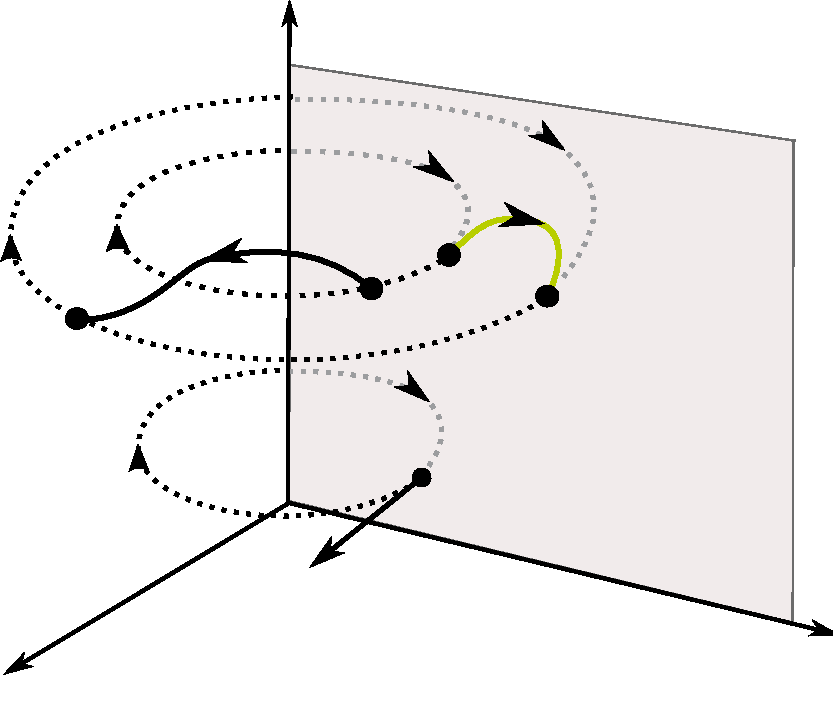
\includegraphics[width=\unitlength]{slice}}%
    \put(0.82835155,0.19007659){\color[rgb]{0,0,0}\rotatebox{-14.84025424}{\makebox(0,0)[lb]{\smash{$\pSRed$}}}}%
    \put(0.06577338,0.24688228){\color[rgb]{0,0,0}\rotatebox{0.0313674}{\makebox(0,0)[lb]{\smash{$\LieEl\,\slicep$}}}}%
    \put(0.53023327,0.21593335){\color[rgb]{0,0,0}\rotatebox{0.0313674}{\makebox(0,0)[lb]{\smash{$\slicep$}}}}%
    \put(0.3184954,0.089285){\color[rgb]{0,0,0}\rotatebox{0.0313674}{\makebox(0,0)[lb]{\smash{$\sliceTan{}$}}}}%
    \put(0.00008985,0.35305068){\color[rgb]{0,0,0}\rotatebox{0.0313674}{\makebox(0,0)[lb]{\smash{$\ssp(\zeit)$}}}}%
    \put(0.69766235,0.41412105){\color[rgb]{0,0,0}\rotatebox{0.0313674}{\makebox(0,0)[lb]{\smash{$\sspRed(\zeit)$}}}}%
    \put(0.06716446,0.70280851){\color[rgb]{0,0,0}\rotatebox{0.0313674}{\makebox(0,0)[lb]{\smash{$\LieEl\,\ssp(\zeit)$}}}}%
  \end{picture}%
\\ %~~~
(b)
  \begin{picture}(1,0.87085079)%
    \put(0,0){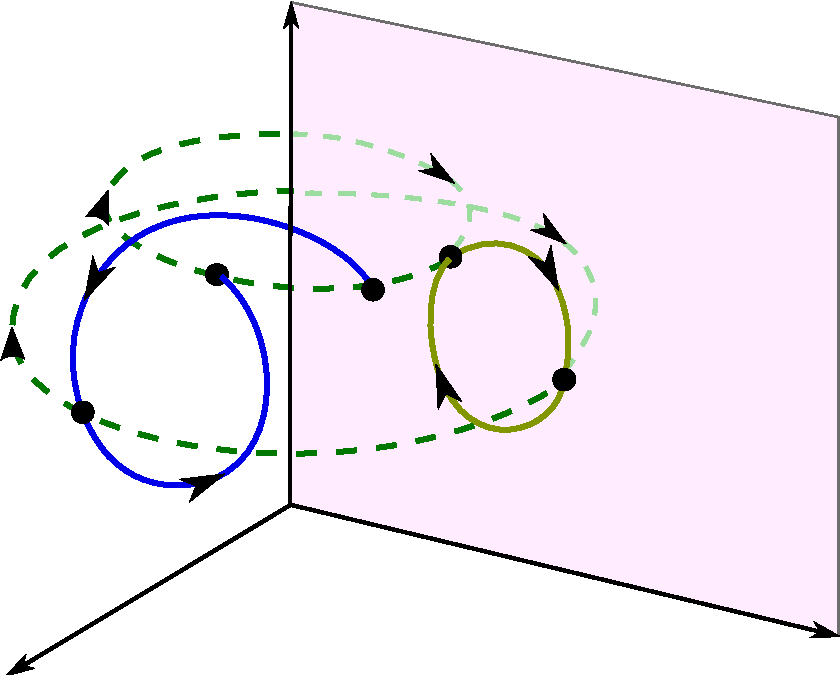
\includegraphics[width=\unitlength]{rpoSlice}}%
    \put(0.82835153,0.19007656){\color[rgb]{0,0,0}\rotatebox{-14.84025432}{\makebox(0,0)[lb]{$\pSRed$}}}%
    \put(0.38925459,0.38713857){\color[rgb]{0,0,0}\rotatebox{0.0313674}{\makebox(0,0)[lb]{\smash{$\ssp(0)$}}}}%
    \put(0.70354118,0.30765314){\color[rgb]{0,0,0}\rotatebox{0.0313674}{\makebox(0,0)[lb]{\smash{$\sspRed(\zeit)$}}}}%
    %\put(0.40171187,0.21813817){\color[rgb]{0,0,0}\rotatebox{0.0313674}{\makebox(0,0)[lb]{\smash{$\LieEl(\zeit)$}}}}%
    \put(0.00068739,0.2359574){\color[rgb]{0,0,0}\rotatebox{0.0313674}{\makebox(0,0)[lb]{\smash{$\ssp(\zeit)$}}}}%
    \put(0.15576193,0.40769256){\color[rgb]{0,0,0}\rotatebox{0.0313674}{\makebox(0,0)[lb]{\smash{$\ssp(\period{})$}}}}%
    \put(0.54113911,0.43476963){\color[rgb]{0,0,0}\rotatebox{0.0313674}{\makebox(0,0)[lb]{\smash{$\sspRed(0)$}}}}%
    %\put(0.06716446,0.70280851){\color[rgb]{0,0,0}\rotatebox{0.0313674}{\makebox(0,0)[lb]{\smash{$\LieEl\,\ssp(\period{})$}}}}%
  \end{picture}%
 \end{center}
 \caption{
The \mslices, a \statesp\ visualization:
(a)
A chart $\pSRed \subset \pS/\Group$ lies in the $(d\!-\!N)$\dmn\
\slice\ hyperplane \refeq{PCsectQ0} normal to $\sliceTan{j}$, which
span the $N$\dmn\ space tangent to the group orbit $\LieEl\,\slicep$
(dotted line) evaluated at the {\template} point $\slicep$. The
hyperplane intersects {all} full \statesp\ group orbits (green
dashes).  The full \statesp\
trajectory $\ssp(\zeit)$ (blue) and the \reducedsp\ trajectory
$\sspRed(\zeit)$ (green) are equivalent up to a `moving frame' rotation
$\ssp(\zeit)=\LieEl(\zeit)\,\sspRed(\zeit)$, where $\LieEl(\zeit)$ is a
shorthand for $\LieEl(\gSpace(\zeit))$.
(b)
In the full \statesp\ a \rpo\ $\ssp(0) \to \ssp(\zeit) \to
\ssp(\period{})$ returns to the group orbit of $\ssp(0)$ after a time
$\period{p}$,  such that $\ssp(0)=\LieEl _p  \ssp
(\period{p})$. A generic \rpo\ quasi-\-periodically fills out what is
topologically a torus (\reffig{fig:CLf01group}\,(b)). In the \slice\
the symmetry-reduced trajectory is periodic, $\sspRed(0) =
\sspRed(\period{p})$.
 }\label{fig:slice}
 \end{figure}

One can write the equations for the flow in the \reducedsp\
$\dot{\sspRed} = \velRed(\sspRed)$ (for details see, , for example,
\refref{DasBuch}) as
    \DB{04-19-2012}{Who actually showed this first... fix reference accordingly.
    \\{\bf Predrag} it's tedious, the history is in the remarks in
    ChaosBook.org continuous.tex, as we say in the introduction - not
    worth getting into this here. Erudition gets into the way here, we
    just want to get to the point as fast and compactly as possible.}
\bea
\velRed(\sspRed) &=& \vel(\sspRed)
     \,-\, \dot{\gSpace}(\sspRed) \, \groupTan(\sspRed)
\label{EqMotMFrame}\\
\dot{\gSpace}(\sspRed) &=& \braket{\vel(\sspRed)}{\sliceTan{}}
                       /\braket{\groupTan(\sspRed)}{\sliceTan{}}
\,
\label{reconstrEq}
\eea
which confines the motion to the \slice\ hyperplane. Thus, the dynamical
system $\{\pS,\map^t\}$ with continuous symmetry \Group\ is replaced by
the {\reducedsp} dynamics $\{\pSRed,\mapRed^t\}$: The velocity in the
full \statesp\ $\vel$ is the sum of $\velRed$, the velocity component in
the \slice\ hyperplane, and $\dot{\gSpace}\,\groupTan$, the velocity
component along the group tangent space. The integral of the {\em
reconstruction equation} for $\dot{\gSpace}$ keeps track of the group
shift in the full \statesp.


%%%%%%%%%%%%%%%%%%%%%%%%%%%%%%%%%%%%%%%%%%%%%%%%%%%%%%%%%%%%%%%%%%%%%
\begin{figure}
   \centering
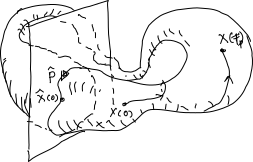
\includegraphics[width=0.30\textwidth]{A29sliceWurst}
   \caption{\label{fig:sliceimage}
\Wurst, sliced.
      Every \slice\ hyperplane cuts every group orbit at least twice (see
      \reffig{fig:slice}), once at the orbit's closest passage to the
      {\template}, and another time at the most distant passage, also
      satisfying the \slice\ condition \refeq{PCsectQ0}. An $\SOn{2}$ \rpo\
      is topologically a torus, so the two cuts are the two \po\ images
      of the same \rpo, the good close one, and the bad distant one, on
      the other side of \chartBord, and thus not in the \slice.
   }
\end{figure}
%%%%%%%%%%%%%%%%%%%%%%%%%%%%%%%%%%%%%%%%%%%%%%%%%%%%%%%%%%%%%%%%%%%%%

The {\template} $\slicep$ should be a generic \statesp\ point in the
sense that its group orbit has the full $N$ dimensions of the group
\Group. The set of the group orbit points \emph{closest} to the
\template\ \slicep\ forms a neighborhood of \slicep\ in which each group
orbit intersects the hyperplane \emph{only once}. A \slice\ hyperplane
captures neighboring group orbits until, for a point $\sspRSing$ not so
close to the \template, the group tangent vector $t(\sspRSing)$ lies in
the \slice\ hyperplane. The group orbits for such points are grazed
tangentially rather than sliced transversally, much like what happens at
the \poincBord\ \refeq{eq:sspRSing} for evolution in time.
This is also a linear condition and defines the \chartBord\ ${\cal
S}$,\rf{SiCvi10,FrCv11} a $(d\!-\!N\!-1)$\dmn\ manifold, which contains
all the points $\sspRSing$ whose group tangents lie in the \slice\
hyperplane, \ie,
\beq
\braket{\sspRSing}{\sliceTan{}} \,=\, 0
      \mbox{ and }
\braket{\groupTan(\sspRSing)}{\sliceTan{}} \,=\, 0
\,.
\label{sliceSingl0}
\eeq
${\cal S}$ also contains all points for which $\groupTan(\sspRSing)=0$.
While for the \PoincSec s \refeq{eq:sspRSing} the analogous points were \eqva\
(captured only if the section cut through them), points with
vanishing group actions belong to invariant subspaces, and -comforting
to know- by its definition every {\chartBord} automatically includes
\emph{all} invariant subspaces.

For the \cLe\ \refeq{eq:CLeR}, the invariant subspace is the 1\dmn\
$z$-axis, with trivial dynamics, $z=-bz$, but in general invariant
subspaces are high-dimensional and have their own dynamics. General
relativists and physicists in general love to work in invariant subspaces
where solutions are highly
symmetric,\rf{SKMacHH09,Christiansen97,lanCvit07,HGC08} as that is easier
than
% PC: sorry Daniel, I prefer saying it as it is. So, now even more strident
    \PCedit{
solving the problem that needs to be solved.\rf{SCD07} Unfortunately,
    }
the dynamics within an invariant subspace has very little to do, if
anything, with the turbulence in the full \statesp\ (for a striking
example, see \refref{ACHKW11}).

\DB{04-19-2012}{Consider moving this whole part on ridges and such to
    \refsect{s:chart}.
    \\{\bf Predrag} It was there originally, but I moved it here because
    in this section (look at the title) we define a single chart, and in
    the next section bind them together into an atlas...
    }
There is yet another, much kinder type of a border: a ridge. Our initial
chart $\pSRed{}^{(1)}$ is a ($d\!-\!1$)\dmn\ hyperplane. If we pick
another {\template} point $\slicep{}^{(2)}$, it comes along with its own
\slice\ hyperplane $\pSRed{}^{(2)}$. Any pair of $(d\!-\!1)$\dmn\ local
\slice\ hyperplanes intersects in a \emph{ridge}, a $(d\!-\!2)$\dmn\
hyperplane {\PoincS} of points $\sspRed^*$ shared by a pair of charts and
thus satisfying the \slice\ condition \refeq{PCsectQ0} for both,
\beq
\braket{\sspRed^*}{\sliceTan{}{}^{(1)}} = 0
\mbox{ and }
\braket{\sspRed^*}{\sliceTan{}{}^{(2)}} = 0
    \,.
\ee{ridge}
This ridge is visualized in \reffig{fig:A29-2slices}\,(c) as a `line' and
in \reffig{fig:A29-1ridge} as a `plane' of intersection of two volumes.
We shall refer to the neighborhood of a \template\ $\slicep{}^{(j)}$
bounded by its {\chartBord} and the ridges to other such linear
neighborhoods as a \emph{chart} $\pSRed{}^{(j)} \subset \pS/\Group$, and
to \refeq{sliceSingl0} and \refeq{ridge} as the {border conditions}.

%%%%%%%%%%%%%%%%%%%%%%%%%%%%%%%%%%%%%%%%%%%%%%%%%%%%%%%%%%%%%%%%
%% A29-2tmplts.* A29-2tmplSl.*
%% Predrag 2012-03-20: see dasbuch/book/FigSrc/inkscape/00ReadMe.txt
%% remember to insert A29-2slices.eps into ChaosBook
 \begin{figure}
 \begin{center}
  \setlength{\unitlength}{0.30\textwidth}
  %% \unitlength = units used in the Picture Environment
(a)\;\;
  \begin{picture}(1,0.92174023)%
    \put(0,0){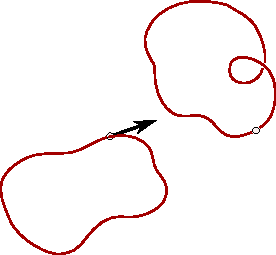
\includegraphics[width=\unitlength]{A29-2tmplts}}%
    \put(0.38186388,0.34995272){\color[rgb]{0,0,0}\makebox(0,0)[lb]{\smash{$\slicep{}^{(1)}$}}}%
    \put(0.41769945,0.50079738){\color[rgb]{0,0,0}\makebox(0,0)[lb]{\smash{$\sliceTan{}{}^{(1)}$}}}%
    \put(0.87339467,0.35886318){\color[rgb]{0,0,0}\makebox(0,0)[lb]{\smash{$\ssp'{}^{(2)}$}}}%
  \end{picture}%
\\
(b)\;\;
  \begin{picture}(1,1.14107266)%
    \put(0,0){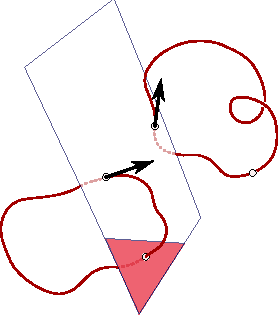
\includegraphics[width=\unitlength]{A29-2tmplSl}}%
    \put(0.54442322,0.48851386){\color[rgb]{0,0,0}\makebox(0,0)[lb]{\smash{$\sliceTan{}{}^{(1)}$}}}%
    \put(0.33649368,0.41474621){\color[rgb]{0,0,0}\makebox(0,0)[lb]{\smash{$\slicep{}^{(1)}$}}}%
    \put(0.41644523,0.62981493){\color[rgb]{0,0,0}\makebox(0,0)[lb]{\smash{$\slicep{}^{(2)}$}}}%
    \put(0.616644,0.84680609){\color[rgb]{0,0,0}\makebox(0,0)[lb]{\smash{$\sliceTan{}{}^{(2)}$}}}%
    \put(0.88017597,0.4261647){\color[rgb]{0,0,0}\makebox(0,0)[lb]{\smash{$\ssp'{}^{(2)}$}}}%
    \put(0.29194797,0.95658666){\color[rgb]{0,0,0}\makebox(0,0)[lb]{\smash{$\pSRed{}^{(1)}$}}}%
  \end{picture}%
 \end{center}
 \caption{\label{fig:A29-2tmplts}
A 2-chart atlas. Sketch
    (a)
depicts two templates $\slicep{}^{(1)}$, $\ssp'{}^{(2)}$, each with its
group orbit. Start with the {\template} $\slicep{}^{(1)}$. All group
orbits traverse its $(d\!-\!1)$\dmn\ \slice\ hyperplane, including the
group orbit of the second {\template} $\ssp'{}^{(2)}$.
    (b)
Replace the second
{\template} by its closest group orbit point $\slicep{}^{(2)}$, \ie, the
point in chart $\pSRed{}^{(1)}$. This is allowed as long as  $\slicep{}^{(2)}$ is
closer than the $\pSRed{}^{(1)}$ {\chartBord} (red region), otherwise an interpolating,
closer template needs to be introduced.
(from \wwwcb{}).
 }
 \end{figure}
%%%%%%%%%%%%%%%%%%%%%%%%%%%%%%%%%%%%%%%%%%%%%%%%%%%%%%%%%%%%%%%%

%%%%%%%%%%%%%%%%%%%%%%%%%%%%%%%%%%%%%%%%%%%%%%%%%%%%%%%%%%%%%%%%
%% A29-2slices.* A29-2charts.*
%% Predrag 2012-03-20: see dasbuch/book/FigSrc/inkscape/00ReadMe.txt
%% remember to insert A29-2slices.eps into ChaosBook
 \begin{figure}
 \begin{center}
  \setlength{\unitlength}{0.40\textwidth}
  %% \unitlength = units used in the Picture Environment
(c)\;\;
  \begin{picture}(1,0.86567815)%
    \put(0,0){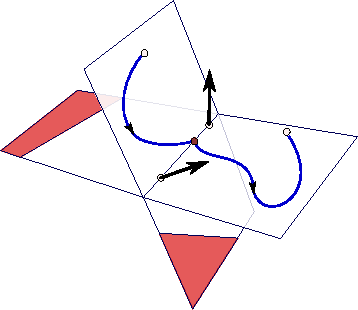
\includegraphics[width=\unitlength]{A29-2slices}}%
    \put(0.3850416,0.38725438){\color[rgb]{0,0,0}\makebox(0,0)[lb]{\smash{$\slicep{}^{(1)}$}}}%
    \put(0.60194012,0.48012421){\color[rgb]{0,0,0}\makebox(0,0)[lb]{\smash{$\slicep{}^{(2)}$}}}%
    \put(0.4042968,0.74412842){\color[rgb]{0,0,0}\makebox(0,0)[lb]{\smash{$\sspRed(0)$}}}%
    \put(0.79647438,0.54627847){\color[rgb]{0,0,0}\makebox(0,0)[lb]{\smash{$\sspRed(\zeit)$}}}%
  \end{picture}%
\\
(d)\;\;
  \begin{picture}(1,0.5127804)%
    \put(0,0){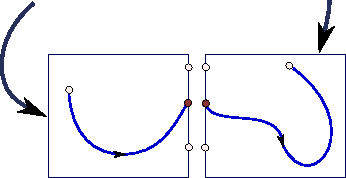
\includegraphics[width=\unitlength]{A29-2charts}}%
    \put(0.16199231,0.03841546){\color[rgb]{0,0,0}\makebox(0,0)[lb]{\smash{$\pSRed{}^{(1)}$}}}%
    \put(0.63051777,0.0374085){\color[rgb]{0,0,0}\makebox(0,0)[lb]{\smash{$\pSRed{}^{(2)}$}}}%
    \put(0.21517269,0.28787637){\color[rgb]{0,0,0}\makebox(0,0)[lb]{\smash{$\sspRed(0)$}}}%
    \put(0.75921701,0.25014044){\color[rgb]{0,0,0}\makebox(0,0)[lb]{\smash{$\sspRed(\zeit)$}}}%
    \put(0.60952792,0.26511997){\color[rgb]{0,0,0}\makebox(0,0)[lb]{\smash{$\slicep{}^{(2)}$}}}%
    \put(0.45827029,0.02997228){\color[rgb]{0,0,0}\makebox(0,0)[lb]{\smash{$\slicep{}^{(1)}$}}}%
  \end{picture}%
 \end{center}
 \caption{\label{fig:A29-2slices}
A 2-chart atlas.
    (c)
Now that the group orbits have been reduced to points, erase them and
consider the two \slice\ hyperplanes through the two {\template s}. As these two
{\template s} are the closest points viewed from either group orbit, they
lie in both \slice\ hyperplanes. However, the two tangent vectors
$\sliceTan{}{}^{(1)}$ and $\sliceTan{}{}^{(2)}$ have different
orientations, so they define two distinct charts
$\pSRed{}^{(1)}$ and $\pSRed{}^{(2)}$ which intersect in the
\emph{ridge}, a hyperplane of dimension $(d\!-\!2)$ (here drawn as a
`line,' and in \reffig{fig:A29-1ridge} as intersection of two `volumes')
shared by the template pair that satisfies both \slice\ conditions
\refeq{ridge}. The chart for the neighborhood of each template (a page of
the atlas in part (d)) extends only as far as this ridge. If the
templates are sufficiently close, the {\chartBord} of each \slice\ hyperplane (red
region) is beyond this ridge, and not encountered by the symmetry-reduced
trajectory $\sspRed(\zeit)$. The reduced trajectory is continuous in the
slice comprised of such charts - it switches the chart whenever it
crosses a ridge.
    (d)
The slice (unique point for each group orbit) is now covered by an atlas
consisting of $(d\!-\!1)$\dmn\ charts $\pSRed{}^{(1)}, \pSRed{}^{(2)},
\cdots$
(from \wwwcb{}).
 }
 \end{figure}
%%%%%%%%%%%%%%%%%%%%%%%%%%%%%%%%%%%%%%%%%%%%%%%%%%%%%%%%%%%%%%%%

%%%%%%%%%%%%%%%%%%%%%%%%%%%%%%%%%%%%%%%%%%%%%%%%%%%%%%%%%%%%%%%%
%% A29-1ridge.*
%% Predrag 2012-03-30: see dasbuch/book/FigSrc/inkscape/00ReadMe.txt
%% remember to insert A29-1ridge.eps into ChaosBook
 \begin{figure}
 \begin{center}
  \setlength{\unitlength}{0.30\textwidth}
  %% \unitlength = units used in the Picture Environment
  \begin{picture}(1,0.89907101)%
    \put(0,0){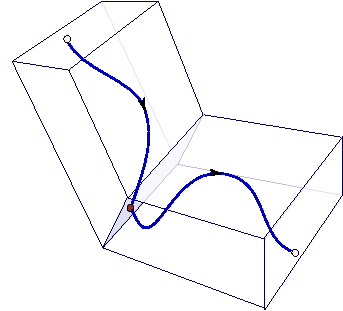
\includegraphics[width=\unitlength]{A29-1ridge}}%
    \put(0.00894598,0.81885604){\color[rgb]{0,0,0}\makebox(0,0)[lb]{\smash{$\sspRed(0)$}}}%
    \put(0.88743345,0.05105926){\color[rgb]{0,0,0}\makebox(0,0)[lb]{\smash{$\sspRed(\zeit)$}}}%
    \put(0.78614059,0.43443027){\color[rgb]{0,0,0}\rotatebox{-25.76142111}{\makebox(0,0)[lb]{\smash{$\pSRed{}^{(2)}$}}}}%
    \put(0.37048948,0.79485578){\color[rgb]{0,0,0}\rotatebox{-61.41291822}{\makebox(0,0)[lb]{\smash{$\pSRed{}^{(1)}$}}}}%
    \put(0.2429401,0.27697318){\color[rgb]{0,0,0}\makebox(0,0)[lb]{\smash{$\sspRed_2$}}}%
    \put(0.47832196,0.33514069){\color[rgb]{0,0,0}\makebox(0,0)[lb]{\smash{$\sspRed_1$}}}%
  \end{picture}%
 \end{center}
 \caption{\label{fig:A29-1ridge}
Here the two charts of \reffig{fig:A29-2slices}\,(c) are drawn as
two $(d\!-\!1)$\dmn\ slabs. Ridge, their $(d\!-\!2)$\dmn\ intersection
can then be drawn as the shaded plane. This hyperplane cuts across the
symmetry-reduced trajectory $\sspRed(\zeit)$ and thus serves as a
\PoincSec\ $\PoincS{}^{(21)}$ that captures all transits from the
neighborhood of {\template} $\slicep{}^{(1)}$ to the neighborhood of
{\template} $\slicep{}^{(2)}$. \PoincSec\ transits are oriented, so
$\sspRed_1$ and $\sspRed_2$ are in the section, but the third point is not
(from \wwwcb{}).
 }
 \end{figure}
%%%%%%%%%%%%%%%%%%%%%%%%%%%%%%%%%%%%%%%%%%%%%%%%%%%%%%%%%%%%%%%%
%%%%%%%%%%%%%%%%%%%%%%%%%%%%%%%%%%%%%%%%%%%%%%%%%
% 2011-09-09, 2012-03-30 Predrag: add BeThMovFr to
%            continuous.tex overheads, and ChaosBook
% replace A27movFrame*.* everywhere
\begin{figure}
 \begin{center}
 \setlength{\unitlength}{0.20\textwidth}
(a) \begin{picture}(1,1.10816305)%
    \put(0,0){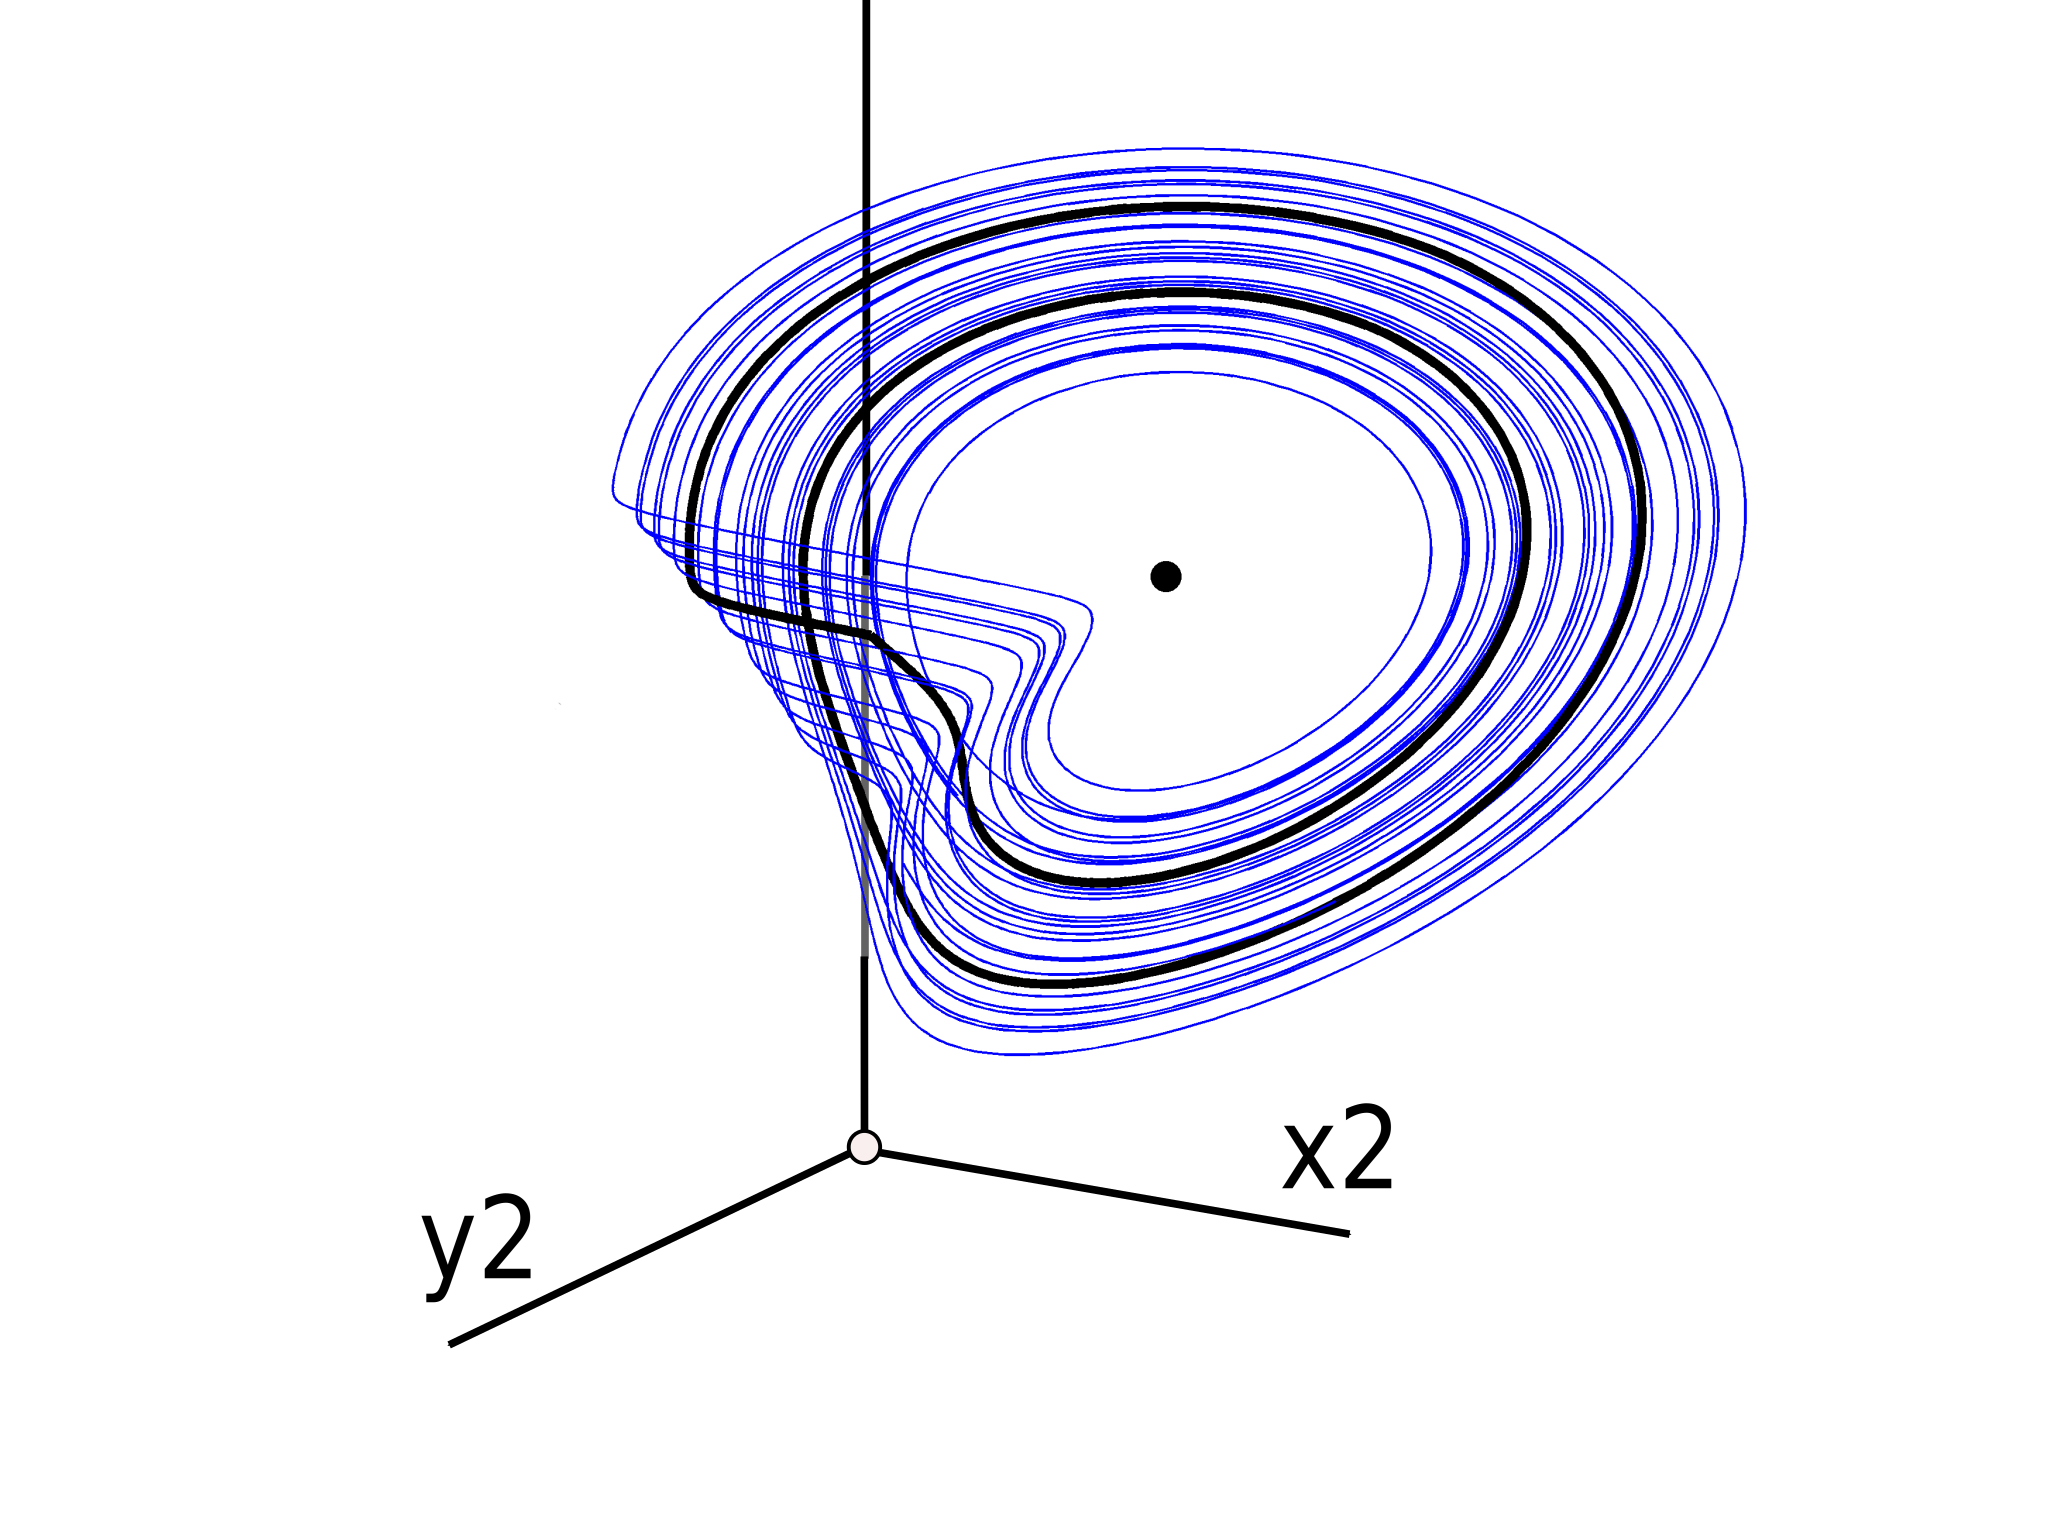
\includegraphics[width=0.8\unitlength]{CLEunsliced}}%
    \put(0.33026558,0.86121262){\color[rgb]{0,0,0}\makebox(0,0)[lb]{\smash{$z$}}}%
    \put(-0.00120214,0.07420659){\color[rgb]{0,0,0}\makebox(0,0)[lb]{\smash{$y_2$}}}%
    \put(0.60769025,0.10190679){\color[rgb]{0,0,0}\makebox(0,0)[lb]{\smash{$x_2$}}}%
  \end{picture}%
(b) \begin{picture}(1,0.87317006)%
    \put(0,0){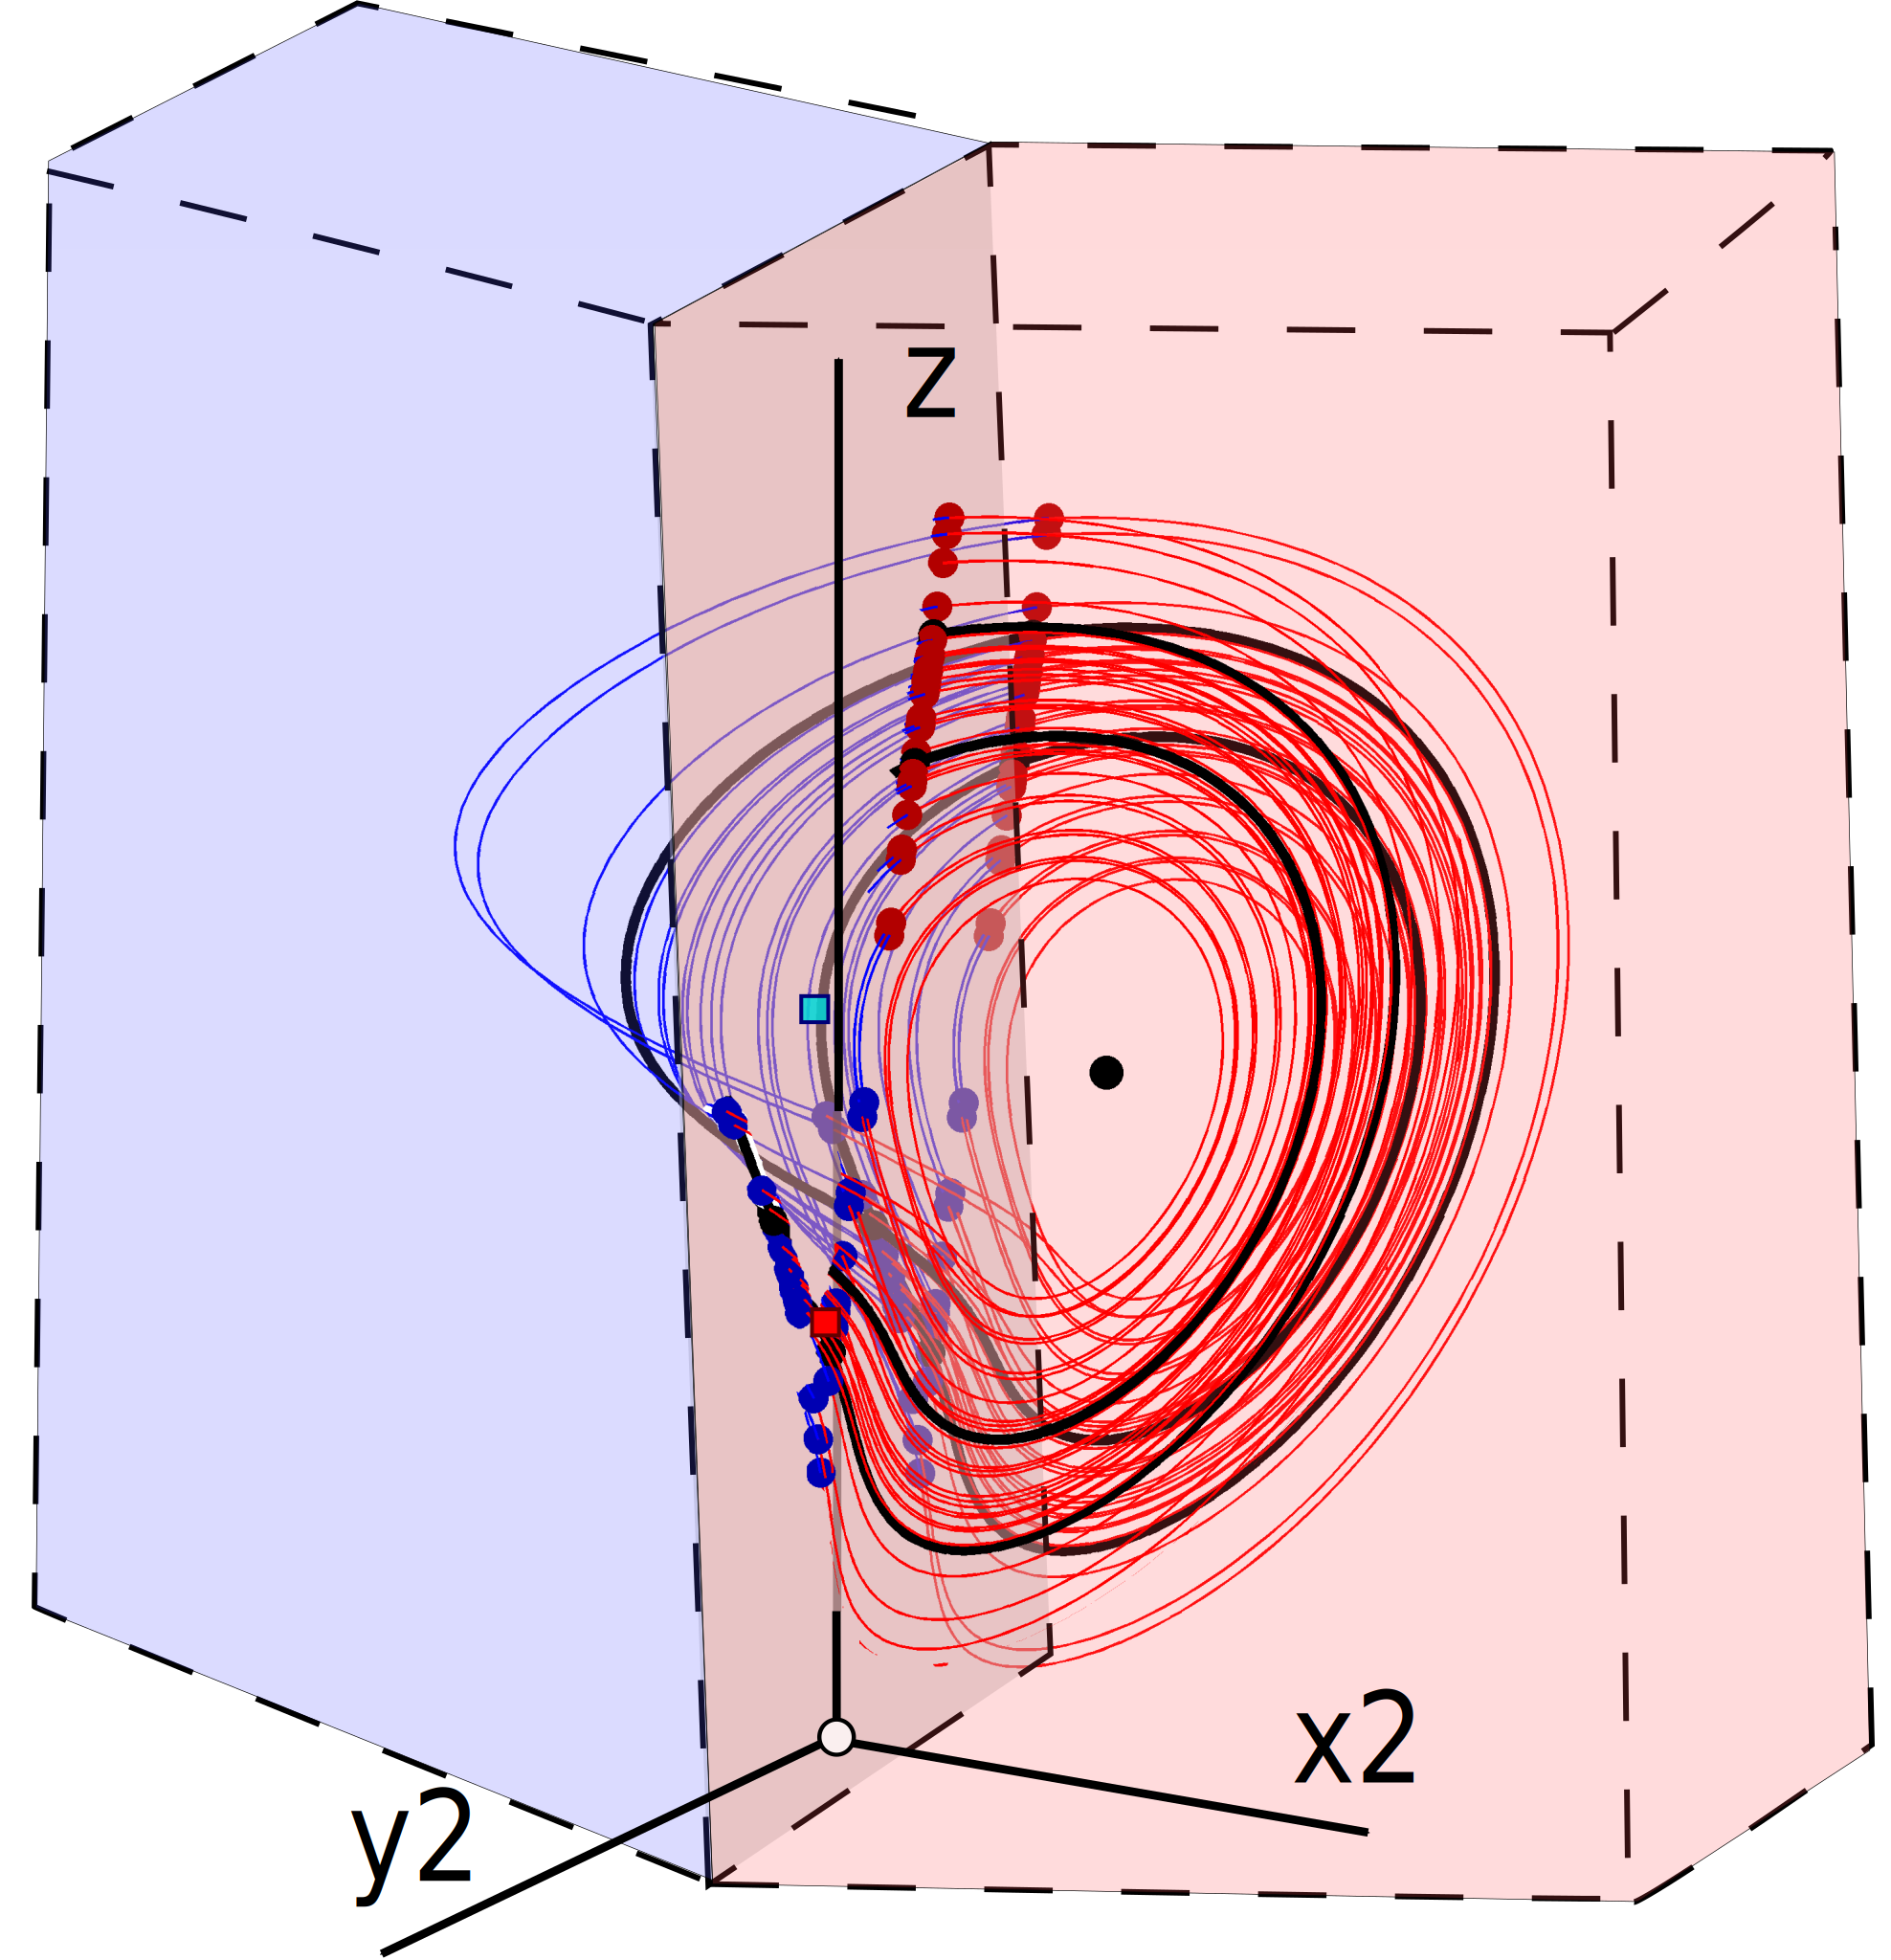
\includegraphics[width=1.2\unitlength]{CLE2slice2na}}%
    \put(0.5407327,0.8152321){\color[rgb]{0,0,0}\makebox(0,0)[lb]{\smash{$z$}}}%
    \put(0.17393473,0.05511623){\color[rgb]{0,0,0}\makebox(0,0)[lb]{\smash{$y_2$}}}%
    \put(0.80432851,0.0789796){\color[rgb]{0,0,0}\makebox(0,0)[lb]{\smash{$x_2$}}}%
  \end{picture}
 \end{center}
  \caption{\label{fig:cLe-2charts}
(a)
Strange attractor of the \cLe, \reffig{fig:CLf01group}\,(a), reduced to a
single \slice\ hyperplane, using as the \template\ the \reqv\ $\slicep =
\ssp_{\REQV{}{1}}$. The attractor exhibits singular jumps due to
forbidden crossings of the \chartBord.
(b)
The 2-chart atlas (sketched in \reffig{fig:A29-1ridge}) of the same
strange attractor encounters no \chartBord s and exhibits no
singularities. The ridge acts as a \PoincSec\ $\PoincS$ with green or
purple ridge points $\sspRed^*$ marking the direction of the crossing.
  }
\end{figure}
%%%%%%%%%%%%%%%%%%%%%%%%%%%%%%%%%%%%%%%%%%%%%%%%%%

\section{Charting the \slice}
\label{s:chart}

Let us summarize the voyage so far: We are charting a curved manifold,
and it would be nice to use tools of differential geometry, but try it in
61,506~dimensions. The only feasible way to chart this space is to (1)
quotient all continuous symmetries, and (2) tile it with flat
$(61,506\!-\!N\!-\!1)$\dmn\ tiles, or charts. We do it step by step,
starting locally, with a set of \template s, and then building chart by
chart to a \emph{\slice} which captures all of the reduced dynamics of
interest (but not all of the possible dynamics). Here are the steps along
the way:

\begin{description}

\item[\Template]
Pick a {\template} $\slicep$ such that $\Group$ acts on it
regularly with a group orbit of dimension $N$.

\item[\Slice\ hyperplane]
The $(d\!-\!N)$-dimensional hyperplane satisfying
\( %beq
\braket{\sspRed}{\sliceTan{a}}=0
\,,
\) %\ee{PCsectQ1}
normal to group transformation directions at the {\template} $\slicep$.
\index{slice}

\item[Moving frame]
For any $\ssp$, the \slice\ condition $\braket{\sspRed}{\sliceTan{}}=0$
on $\ssp = \LieEl(\gSpace)\sspRed$ determines the moving frame, \ie, the
group action $\LieEl(\gSpace)$ that brings $ \ssp$ into the \slice\
hyperplane.
\index{moving frame}

\item[\ChartBord]
The set of points in \slice\ hyperplane whose group orbits are grazed
tangentially, with both points $\sspRSing$ and their group tangents
$\groupTan(\sspRSing)$  in the \slice\ hyperplane,
$\braket{\sspRSing}{\sliceTan{}} \,=\,
\braket{\groupTan(\sspRSing)}{\sliceTan{}} \,=\, 0 \,.$

    \PCedit{
\item[Flow invariant subspace]
If a subset or all of the group tangents of a \chartBord\ point
$\sspRSing$ vanish, $\groupTan_a(\sspRSing)=0$, its time  trajectory
remains within a flow-invariant subspace for all times.
        }

\item[Ridge]
A hyperplane of points $\sspRed^* \in \PoincS{}^{(21)}$ formed by the
intersection of a pair of \slice\ hyperplanes $\pSRed{}^{(1)}$ and
$\pSRed{}^{(2)}$. Ridge is a \PoincSec\ $\PoincS{}^{(ij)}$ that serves as
a toll bridge, crossed by any transit from a chart $\pSRed{}^{(j)}$ to an
adjacent chart $\pSRed{}^{(i)}$.

\item[Chart]
The neighborhood of a \template\ $\slicep{}^{(j)}$, bounded by the
{\chartBord} and the ridges to other linear neighborhoods, comprises
a \emph{chart} $\pSRed{}^{(j)} \subset \pS/\Group$. The borders ensure
that there is no more than one oriented group orbit traversal per chart;
a group orbit either pierces one chart, or no charts at all.

\item[Atlas]
A set of $(d\!-\!N)$\dmn\ contiguous charts $\pSRed{}^{(1)},
\pSRed{}^{(2)}, \cdots$

\item[\Slice]
Let $\Group$ act on a $d$-dimensional manifold $\pS$, with group
orbits of dimension $N$ or less. A \emph{\slice} is a $(d\!-\!N)$
dimensional submanifold $\pSRed$ such that all group orbits that
intersect $\pSRed$ do so transversally and only once.

\end{description}

In literature\rf{Mostow57,Pal61,GuiSte90} `\slice' refers to any
co-dimension~$N$ manifold that slices transversally. Here we have defined
an atlas over a \slice\ constructively but more narrowly, as a contiguous
set of flat charts, with every group orbit accounted for by the
atlas sliced only once, and belonging to a single chart. A \slice\ is not
global, it slices only the group orbits in an open neighborhood of the
\statesp\ region of interest.

The physical task is to, for a given dynamical flow, pick a set of
qualitatively distinct {\template s} (for a turbulent pipe
flow there might be one typical of 2-roll states, one for 4-roll states, and so on)
which together provide a good atlas for the region of $\pS/\Group$
explored by chaotic trajectories.

The rest is geometry of hyperplanes, nothing to do with dynamics. Group
orbits $\pS_{\slicep}$, group tangents $\groupTan(\slicep)$, and the
associated charts are purely group-theoretic, linear concepts. The
\slice, \chartBord\ and ridge conditions \refeq{PCsectQ0},
\refeq{eq:chartBord} and \refeq{ridge} are all linear conditions which
depend on the ray defined by the \template\ \slicep, not its magnitude.
Checking whether the {\chartBord} is on the far side of the ridge between
two \slice\ hyperplanes is a linear computation; for a symmetry-reduced
trajectory moving in $\pSRed{}^{(1)}$ chart one only has to keep checking
the sign of
\beq
\braket{\sspRed(\zeit)}{\sliceTan{}{}^{(2)}}
\,.
\ee{eq:chartBord}
Once the sign changes, the ridge has been crossed, and from then on
the trajectory should be reduced to the $\pSRed{}^{(2)}$ chart.
How this works in practice is illustrated by the 2-chart atlas of
\cLe, see \reffig{fig:cLe-2charts}.

How the charts are put together is best told as a graphic tale, in the 5
frames of Figs.~\ref{fig:A29-2tmplts}, \ref{fig:A29-2slices} and
\ref{fig:A29-1ridge}, and then illustrated by contrasting the mess of the
\cLe\ strange attractor \reffig{fig:CLf01group}\,(a) to the elegance of
its 2-chart atlas, \reffig{fig:cLe-2charts}\,(b).

Two concluding remarks on what \slice s \emph{are not}:

(1) Symmetry reduction is not a dimensional-reduction scheme, or a
projection on a fewer coordinates, or flow modeling by fewer degrees of
freedom: It is a local change of coordinate with one (or $N$)
coordinates pointing along the phase directions. No information is lost
by symmetry `reduction', one can go freely between solutions in the full
and reduced \statesp s by integrating the associated {reconstruction
equations} \refeq{reconstrEq}.

(2) An atlas is \emph{not needed} for Newton determination of a single
invariant solution, or a study of its bifurcations.\rf{golubII} Any local
section and slice plus time and shift constraints does the job. 60,000
\rpo s can be computed\rf{SCD07} this way. Once we have more than one
invariant solution, the question is: How is this totality of solutions
interrelated? and for that a good atlas is a necessity.


\section{Bridges to nowhere}
\label{s:bridge}
    % kvetches, still to be written

Everybody encounters a symmetry sooner or later, so the literature on
symmetry reduction is vast (for a historical overview, see remarks in
ChaosBook.org and \refref{SiCvi10}). Before asking - why the \mslices\
and not my [...]? a brief tour of the graveyard of obvious ideas and pet
symmetry reduction schemes is called for. They all have one thing in
common: they will not work for high-dimensional systems.

To start with: if you are a master of quantum-mechanics or QFT symmetries
and their linear irreducible representations,\rf{PCgr} you may leave your
baggage at the door - the way symmetries act on nonlinear systems is much
subtler, as we tried to show in this pictorial tour. The same for masters
of bifurcations\rf{ruell73,golubII} - linear theory works quite well at
the bifurcations, not so globally.

There are purely group-theoretical approaches, with no dynamics to inform
them. For $\SOn{2}$, an obvious idea is to go to polar coordinates. The
simplest nonlinear examples\rf{AGHO288} already run into $r_j \to 0$ type
of singularities, and it is not altogether clear how one would rewrite
the \NSe\ in such a format, or integrate them numerically. For pipe
flows, one would need cylindrical Bessel eigenbases, which are never used
in numerical work. A more sophisticated  approach would be to rewrite the
dynamics in terms of invariant polynomial bases, described lucidly in
\refref{GL-Gil07b}, with equivariant \statesp\ coordinates
$(x_1,x_2,x_3,...,x_d)$ replaced by invariant polynomial basis
$(u_1,u_2,u_3,...,u_m)$. As the dimension of the problem increases, the
number of these polynomials grows, and so does the number of syzygies,
the nonlinear relations amongst them. There is no guiding principle for
picking a set of such polynomials, and no practical way to implement the
scheme\rf{gatermannHab} for high-dimensional flows:
why would one replace the 61,506 equivariant \statesp\ coordinates of
hydrodynamic turbulence with a vast number of invariant polynomials?

There are approaches informed by dynamics, foremost among them being the
method of {co-moving frames}. Visualizing a single `relative' trajectory
in its co-moving frame, \ie, moving with that solution's mean
{\phaseVel}, is useful if one is concerned with that individual solution
and the tiny \rpo s (modulated-amplitude waves) that have bifurcated off
it.\rf{duguet08,mellibovsky11} A co-moving frame is useless, however, if
we are concerned with studying collections of these trajectories, as each
solution travels with its own mean {\phaseVel}, and there is no single
co-moving frame that can simultaneously reduce \emph{all} traveling
solutions. The \slice\ that we construct here is not `co-moving,' but
\emph{emphatically} stationary.

There exist sophisticated approaches to reducing symplectic symmetry of
mechanics of a three dimensional rigid body,\rf{MaWe74} or using Lie
symmetry reduction to derive Eulerian velocity fields from Lagrangian
trajectories.\rf{MorrGree80} They do not appear to work for problems
considered here, and anyway, the goal is different. Rather than to reduce
a particular set of equations, we seek to formulate a computationally
straightforward and general method of reducing any continuous symmetry,
for any high-dimensional chaotic/turbulent flow. One should also note
that ``symmetry reduction'' in general relativity\rf{SKMacHH09} and Lie
theory often implies restricting one's solution space to a subspace of
higher symmetry; here we always work in the full \statesp.

There is, however, one intriguing, obvious and physically informed
contender.
    \PCedit{
In mechanics and field theory it is natural to separate the flow {\em
locally} into group dynamics and a transverse, `horizontal'
flow,\rf{Smale70I,AbrMars78} by the `method of
connections,'\rf{rowley_reduction_2003} see \reffig{fig:BeThMconnect}.
    }
It is the group dynamics cousin of the strobing method of \refsect{s:cut}
and does not reduce the dynamics to a lower-dimensional \reducedsp\
$\pS/\Group$. In field theory the freedom of choosing moving frames of
\reffig{fig:BeThMovFr} is called ``gauge freedom,'' and a particular
prescription of choosing a frame is called ``gauge fixing,'' or a
``gauge.'' The classical dynamics meaning of the ``method of
connections'' is clearest in the work of Shapere and
Wilczek:\rf{ShWi89a,ShWi06} one can observe a swimmer (or our dancer)
from a fixed \slice\ frame, or bring her back to observe only the
shape-changing dynamics, no drifting. Left to herself, she will reemerge
in the same pose someplace else: that shift is called a ``geometrical
phase,'' which -while accruing it is the whole point of swimming- had not
played any role our discussion of symmetry reduction. Conversely, most gauge
choices in quantum field theory are covariant, and while that suffices to
regularize path integrals, the \mslices\ says that this is no symmetry
reduction at all, and it yields no insight into the geometry of nonlinear
flows.


%%%%%%%%%%%%%%%%%%%%%%%%%%%%%%%%%%%%%%%%%%%%%%%%%%%%%%%%%%%%%%%%%%%%%
\begin{figure}
   \centering
  \setlength{\unitlength}{0.20\textwidth}
(a)~~~
  \begin{picture}(1,0.98073806)%
    \put(0,0){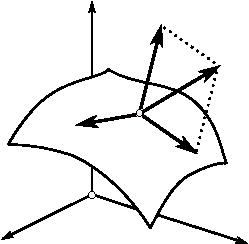
\includegraphics[width=\unitlength]{A28tangents}}%
    \put(0.8635648,0.73622308){\color[rgb]{0,0,0}\makebox(0,0)[lb]{\smash{$\vel$}}}%
    \put(0.49893205,0.86039365){\color[rgb]{0,0,0}\makebox(0,0)[lb]{\smash{$\vel_{\bot}$}}}%
    \put(0.27198728,0.5378933){\color[rgb]{0,0,0}\makebox(0,0)[lb]{\smash{$\groupTan_1$}}}%
    \put(0.58493215,0.33483773){\color[rgb]{0,0,0}\makebox(0,0)[lb]{\smash{$\groupTan_2$}}}%
    \put(0.54959234,0.21257862){\color[rgb]{0,0,0}\makebox(0,0)[lb]{\smash{$\LieEl\ssp$}}}%
  \end{picture}%
(b)~~~
  \begin{picture}(1,0.98655417)%
    \put(0,0){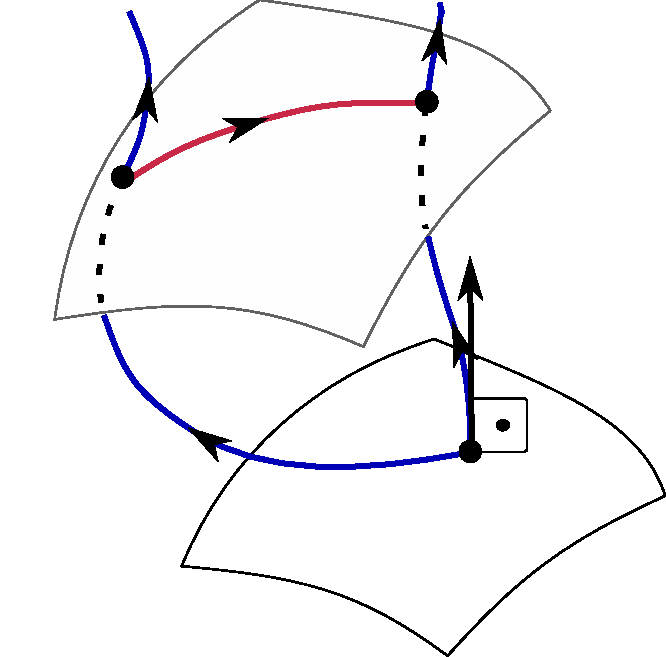
\includegraphics[width=\unitlength]{BeThMconnect}}%
    \put(0.20559239,0.64023845){\color[rgb]{0,0,0}\rotatebox{0.0313674}{\makebox(0,0)[lb]{\smash{$\ssp(\zeit)$}}}}%
    \put(0.68383186,0.20519203){\color[rgb]{0,0,0}\rotatebox{0.0313674}{\makebox(0,0)[lb]{\smash{$\ssp(0)$}}}}%
    \put(0.67475925,0.8109461){\color[rgb]{0,0,0}\rotatebox{0.0313674}{\makebox(0,0)[lb]{\smash{$\sspRed(\zeit)$}}}}%
    \put(0.35760559,0.8662057){\color[rgb]{0,0,0}\rotatebox{0.0313674}{\makebox(0,0)[lb]{\smash{$\LieEl(\zeit)$}}}}%
    \put(0.70884327,0.61850672){\color[rgb]{0,0,0}\rotatebox{0.0313674}{\makebox(0,0)[lb]{\smash{$\vel_{\bot}$}}}}%
  \end{picture}%
   \caption{\label{fig:BeThMconnect}
    (a)
By equivariance $\vel(\ssp)$ can be replaced by $\vel_\bot(\ssp)$, the
velocity normal to the group tangent directions at \statesp\ point $\ssp$.
    (b)
Method of connections replaces $\vel(\sspRed)$ at every instant
$\sspRed =\sspRed(\zeit)$ by $\vel_\bot(\sspRed)$, so in
$\sspRed(\zeit)$ covariant frame there is no motion along the group
tangent directions.
}
\end{figure}
%%%%%%%%%%%%%%%%%%%%%%%%%%%%%%%%%%%%%%%%%%%%%%%%%%%%%%%%%%%%%%%%%%%%%


\section{Conclusions}
\label{s:concl}

As turbulent flow evolves, every so often we catch a glimpse of a
familiar structure. For any finite spatial resolution and time, the flow
follows an unstable {\cohStr} belonging to an alphabet of representative
states, here called `\template s'. However, in the presence of
symmetries, near recurrences can be identified only if shifted both in
time and space.

In the method of sections (along time direction) and slices (along
spatial symmetry directions), the identification of physically close
states is achieved by cutting the group orbits with a finite set of
hyperplanes, one for each continuous parameter, with each time trajectory
and group orbit of symmetry-equivalent points represented by a single
point, its  section and \slice. The \mslices\ is akin to (but distinct
from) cutting across trajectories by means of sections. Both methods
reduce continuous symmetries: one sections the continuous-time
trajectories, the other slices the layers of the onion formed by
group-orbits. Both are triggered by analogous conditions: oriented piercing of
the section and oriented piercing of the slice. Just as a \PoincSec\ goes
bad, the \slice\ hyperplane goes bad the moment transversality is lost. A
slice, however, is emphatically \emph{not} a \PoincSec. Instead it
replaces a trajectory by a continuous symmetry-reduced trajectory,
whereas a \PoincSec\ replaces a continuous time trajectory by a discrete
sequence of points.

%    \BR{2012-4-15 My stab at this paragraph:
%    \PC{2012-4-15 went back to my version, mostly
Note also that symmetry reduction is not a dimensional-reduction scheme,
or flow modeling by fewer degrees of freedom: the full dimensionality of
the original dynamical system is retained. No information is lost, as
one can go freely between solutions in the full and reduced \statesp s by
integrating the associated {reconstruction equation} \refeq{reconstrEq}.

The main lesson of the visual tour undertaken above is that if a
dynamical problem has a continuous symmetry, the symmetry \emph{must} be
reduced before any detailed analysis of the flow's \statesp\ geometry can
take place. So far, this has only been achieved for transitionally
turbulent numerical pipe flows\rf{ACHKW11} resulting in the discovery of
the first \rpo s embedded in turbulence. In the future it should be the
first step in the analysis of any turbulent data, numerical\rf{CvGr12} or
experimental.\rf{BCS12} Once symmetry reduction is achieved, all
solutions of a turbulent flow can be plotted together, as one happy
family: all symmetry-equivalent states are represented by a single point,
families of solutions are mapped to a single solution, \reqva\ become
\eqva, \rpo s become \po s, and most importantly, the analysis of the
global dynamical system in terms of invariant solutions and their stable
/ unstable manifolds can now commence.

\begin{acknowledgments}
This article answers the questions asked after the talk given at
Kyoto 2011 IUTAM Symposium on ``50 Years of Chaos: Applied and Theoretical.''
We are indebted to
S.~Flynn,
S.~Froehlich,
S.A.~Solla,
and
R.~Wilczak
for inspiring discussions.
P.C.\ thanks G.~Robinson,~Jr.\ for support,
Max-Planck-Institut f\"ur Dynamik und Selbstorganisation,
G\"ottingen for hospitality,
and the Nieders\"achsischen Knackwurst and Bayerische Hefeweizen for
making it all possible.
    \DB{ASAP}{D.B.\ was supported by NSF grant ???.}
P.C.\ was partly supported by NSF grant DMS-0807574
and
2009 Forschungspreis der Alexander von Humboldt-Stiftung.
\end{acknowledgments}


\bibliography{../bibtex/siminos}


\ifdraft
    \onecolumngrid

    \newpage
\input figures
    \newpage
\input flotsam
    \newpage
    \section{Daily blog, point by point}
    \label{chap:atlas}
\input ../blog/atlas
\fi

\end{document}
